\documentclass[twocolumn,10pt,amsmath,amssymb,floatfix]{revtex4-2}

\usepackage[T1]{fontenc}
\usepackage{amsthm,mathtools}
\usepackage{booktabs}
\usepackage{array}
\usepackage{graphicx}
\usepackage{xcolor}
\usepackage{microtype}
\usepackage{enumitem}
\usepackage[colorlinks=true,linkcolor=blue!55!black,citecolor=blue!55!black,urlcolor=blue!55!black]{hyperref}

\theoremstyle{plain}
\newtheorem{theorem}{Theorem}
\newtheorem{proposition}[theorem]{Proposition}
\newtheorem{lemma}[theorem]{Lemma}
\newtheorem{corollary}[theorem]{Corollary}

\theoremstyle{definition}
\newtheorem{definition}[theorem]{Definition}
\newtheorem{remark}[theorem]{Remark}

\newcommand{\dd}{\mathrm{d}}
\newcommand{\ii}{\mathrm{i}}
\newcommand{\ee}{\mathrm{e}}
\newcommand{\Tr}{\operatorname{Tr}}
\newcommand{\sgn}{\operatorname{sgn}}
\newcommand{\normF}[1]{\left\lVert #1 \right\rVert_F}
\newcommand{\PS}{P_S}
\newcommand{\PT}{P_T}
\newcommand{\HRP}{H_{\mathrm{RP}}}
\newcommand{\HZ}{H_Z}
\newcommand{\HHF}{H_{\mathrm{HF}}}
\newcommand{\Hex}{H_{\mathrm{ex}}}
\newcommand{\Hdip}{H_{\mathrm{dip}}}
\newcommand{\DeltaPhi}{\Delta\Phi_S}
\newcommand{\xiflip}{\xi_{\mathrm{flip}}}
\newcommand{\leanid}[1]{{\footnotesize\ttfamily\def\_{\textunderscore\allowbreak}#1}}

\begin{document}
\setlength{\dbltextfloatsep}{10pt plus 2pt minus 2pt}
\setlength{\dblfloatsep}{8pt plus 2pt minus 2pt}
\setlength{\emergencystretch}{1.8em}

\title{Fourth-Moment Commutator Protection, Five-Channel Liouvillian Scaling, and Non-Commuting Colored-Bath Dynamics in Radical-Pair Magnetoreception}

\author{Mehardeep Singh}
\email{mehardeep.sim@gmail.com}
\affiliation{Sri Chaitanya Educational Institutions}

\date{}

\begin{abstract}
Why does a weak geomagnetic field ($\sim 50\,\mu\text{T}$) modulate radical-pair singlet yields despite strong environmental spin relaxation, and when do phenomenological relaxation models misrepresent local non-commuting spin baths? We resolve both questions using exact commutator identities, time-reversal symmetry, Feshbach--Schur resolvent asymptotics, 45-digit Liouvillian and Auxiliary Density Operator (ADO) numerics, and pure Lean~4.16.0 formal proofs. Because the electronic Zeeman Hamiltonian $\HZ(\hat{\mathbf{b}})$, isotropic exchange $\Hex$, and any symmetric electron--electron dipolar interaction $\Hdip = \mathbf{S}_1\cdot\mathbf{D}\cdot\mathbf{S}_2$ ($\mathbf{D}^\top = \mathbf{D}$) commute identically with the singlet projector $\PS$ for arbitrary nuclear spin architectures, both the zeroth and second nested-commutator moments $M_0 = 1$ and $M_2 = \sum_k \frac{I_k(I_k+1)}{6}\Tr(\mathbf{A}_k\mathbf{A}_k^\top)$ are strictly independent of field orientation $\hat{\mathbf{b}}$, exchange $J_{\mathrm{ex}}$, and dipolar tensor $\mathbf{D}$. Directional sensitivity first enters at the fourth commutator moment: by antiunitary spin time-reversal orthogonality between the $T$-odd Zeeman commutator and all $T$-even internal spin--spin commutators, $M_4(\hat{\mathbf{b}}) - M_4(\hat{\mathbf{n}}_0) = \sum_k \frac{I_k(I_k+1)}{6}\omega_L^2 \bigl(\hat{\mathbf{n}}_0^\top\mathbf{A}_k\mathbf{A}_k^\top\hat{\mathbf{n}}_0 - \hat{\mathbf{b}}^\top\mathbf{A}_k\mathbf{A}_k^\top\hat{\mathbf{b}}\bigr)$, strictly invariant under arbitrary $J_{\mathrm{ex}}$ and $\mathbf{D} = \mathbf{D}^\top$, reducing for an axial hyperfine tensor to $\frac{I(I+1)}{6}\omega_L^2(A_\parallel^2 - A_\perp^2)\sin^2\theta$. Under global commuting relaxation ($\xi = \gamma/k_{\mathrm{rec}} \gg 1$), this \emph{Fourth-Moment Commutator Protection} collapses Markovian anisotropy as $\DeltaPhi(\mu=1) = \Theta(\xi^{-5})$---preceded by a high-order \emph{sign-flip blind spot} ($\xiflip = 1.3233$ in the canonical $8\times 8$ system; $\xiflip = 412.06$ in $36\times 36$ physical $50\,\mu\text{T}$ $\mathrm{FAD}^{\bullet-}\text{--}\mathrm{Z}^{\bullet}$, alongside $\xiflip = 685.02$ for local isotropic $\mathbf{S}_1$)---whereas completely monotonic Mittag--Leffler memory $E_\mu(-(\gamma t)^\mu)$ ($0<\mu<1$) yields $\Theta(\xi^{-\mu})$ decay without sign flips for $\mu \le 0.85$ in the canonical $8\times 8$ model. Local non-commuting Markovian relaxation splits this universality into five distinct Feshbach--Schur dark-manifold exponents: singlet--triplet dephasing gives $\Theta(\xi^{-2})$ via Zeno cancellation of $M_2$ and a dark-triplet iterate; single-radical isotropic noise on $\mathbf{S}_1$ gives $\Theta(\xi^{-4})$ via a four-bright-step Schur cascade (vs.\ $\Theta(\xi^{-5})$ on both radicals or on $\mathbf{S}_2$ at $J_{\mathrm{ex}}=0$, $\Hdip=0$); two-radical uniaxial dephasing ($S_{1z}+S_{2z}$) gives $\Theta(\xi^{-1})$; single-radical uniaxial dephasing ($S_{1z}$) saturates at $\Theta(\xi^0)$ ($\DeltaPhi^\infty \approx 0.1642$ canonical, $0.2467$ at $50\,\mu\text{T}$); and asymmetric Haberkorn recombination ($k_T/k_S \in [0.1,10]$) preserves trace normalization ($\max|\Phi_S+\Phi_T-1|\le 8.2\times 10^{-43}$) and every asymptotic exponent. Finally, embedding positive $K=8$ Prony fits ($\le 0.69\%$ kernel error) to non-commuting $1/f^\alpha$ magnetic noise $C(t) = \sigma^2(1+t/\tau_c)^{-\mu}$ inside Tanimura--Kubo ADOs cross-checked against exact integrated-OU Monte Carlo ensembles on both $8\times 8$ and $36\times 36$ $50\,\mu\text{T}$ $\mathrm{FAD}^{\bullet-}\text{--}\mathrm{Z}^{\bullet}$ models isolates the exact breakdown of motional narrowing ($\sigma\tau_c \gtrsim 1$) and clarifies quantitatively where broadband $1/f^\alpha$ noise differs from matched single-mode Ornstein--Uhlenbeck noise versus where both converge to the quasi-static $\sigma^{-2}$ plateau. All core spin-projector, arbitrary multi-nucleus $M_0/M_2/M_4$ (arbitrary attachment $e_k \in \{1,2\}$ and arbitrary symmetric dipolar $\mathbf{D}$), Lorentzian resolvent, and reduced dark-manifold theorems (364 authored public theorems, 501 authored total, 560 kernel-audited public declarations including 69 headline theorems; 5,991 lines) are machine-checked without external axioms or \texttt{sorry} in pure Lean~4.16.0.
\end{abstract}

\maketitle

%==============================================================================
\section{Introduction}
%==============================================================================

The radical-pair mechanism provides the leading biophysical candidate for the avian inclination compass, proposing that coherent singlet--triplet interconversion in photoinduced cryptochrome $\mathrm{FAD}^{\bullet-}\text{--}\mathrm{TrpH}^{\bullet+}$ (or reference-probe $\mathrm{FAD}^{\bullet-}\text{--}\mathrm{Z}^{\bullet}$) radical pairs renders spin-selective chemical yields sensitive to the geomagnetic inclination $\theta$~\cite{Schulten1978ZPC,Steiner1989ChemRev,Timmel1998MolPhys,Ritz2000BJ,Ritz2004Nature,Lee2014JRSocInterface,Hore2016ARB,Xu2021Nature}. Because Earth's magnetic field ($B_0 \approx 50\,\mu\text{T}$, electron Larmor frequency $\omega_L \approx 8.80\,\text{rad}\,\mu\text{s}^{-1}$) is orders of magnitude weaker than thermal energies and smaller than dominant $^{14}\text{N}$ hyperfine couplings ($A_{\mathrm{N5},\parallel} \approx 309\,\text{rad}\,\mu\text{s}^{-1}$), sustaining directional contrast against environmental spin relaxation and electron--electron dipolar interactions has attracted sustained theoretical and experimental scrutiny~\cite{Efimova2008BJ,Kominis2009PRE,Jones2010CPL,Cai2010PRL,Gauger2011PRL,Tiersch2012PhilTrans,Hogben2012PRL,Worster2016JCP,Hiscock2016PNAS,Kattnig2016PCCP,Kattnig2016NJP,Fay2018JCP,Fay2019JCP,Fay2020Faraday,Babcock2020JPCL}.

Across this literature, however, seemingly minor differences in how relaxation and environmental memory are modeled yield conflicting scaling laws under strong noise ($\xi := \gamma/k_{\mathrm{rec}} \gg 1$). Second-order perturbation intuition suggests $O(\xi^{-1})$ suppression, phenomenological singlet--triplet dephasing models give slower $O(\xi^{-2})$ Zeno scaling~\cite{Dellis2012Biosystems,Tiersch2012PhilTrans}, isotropic local or global Markovian channels drop far more steeply~\cite{Worster2016JCP,Kattnig2016PCCP} while asymmetric local relaxation can preserve or even enhance sensitivity~\cite{Tiersch2012PhilTrans,Kattnig2016NJP}, and non-Markovian colored baths exhibit strong departures from Redfield theory~\cite{Fay2019JCP,Tanimura2020JCP} alongside algebraic tails in fractional models~\cite{Metzler2000PR,Sokolov2001PRE,Pollard1948BAMS,Gorenflo2002FCAA}. In particular, extrapolating Redfield or Markovian Lindblad rates $\gamma_{\mathrm{eff}} = 2\sigma^2\tau_{\mathrm{int}}$ beyond the motional-narrowing regime ($\sigma\tau_c \gtrsim 1$)---an effect highlighted via Nakajima--Zwanzig and HEOM studies of radical-pair relaxation by Fay \emph{et~al.}~\cite{Fay2019JCP}---or treating phenomenological scalar commuting envelopes $E_\mu(-(\gamma t)^\mu)$ as proxies for biological cryptochrome noise conflates two physically distinct mechanisms: (i) algebraic survival tails of global commuting relaxation versus (ii) breakdown of motional narrowing and spectral-weight redistribution in local, non-commuting colored magnetic fields with finite RMS strength $\sigma$ and ultraviolet correlation time $\tau_c$~\cite{Schulten1978JCP,Kattnig2016PCCP,Kattnig2016NJP,Fay2019JCP,Fay2020Faraday}.

In this paper, we establish a unified, mathematically exact, and formally verified framework separating these mechanisms cleanly across three complementary levels:

\begin{enumerate}[leftmargin=1.4em,itemsep=1pt,topsep=3pt]
\item \textbf{Fourth-Moment Commutator Protection with Exchange and Dipolar Couplings (Sec.~\ref{sec:moments}):} We prove that for arbitrary multi-nucleus spin Hamiltonians $\HRP(\hat{\mathbf{b}}) = \HZ(\hat{\mathbf{b}}) + \HHF + \Hex + \Hdip$ with arbitrary real symmetric electron--electron dipolar tensor $\mathbf{D}^\top = \mathbf{D}$, the vanishing commutators $[\HZ,\PS] = [\Hex,\PS] = [\Hdip,\PS] = 0$ force both $M_0 = 1$ and $M_2 = \sum_k \frac{I_k(I_k+1)}{6}\Tr(\mathbf{A}_k\mathbf{A}_k^\top)$ to be strictly independent of $(\theta,\phi)$, $J_{\mathrm{ex}}$, and $\mathbf{D}$. By antiunitary total-spin time-reversal orthogonality, directional anisotropy enters strictly at $M_4(\hat{\mathbf{b}}) - M_4(\hat{\mathbf{n}}_0)$, which is likewise \emph{strictly invariant} under arbitrary $J_{\mathrm{ex}}$ and $\mathbf{D}^\top = \mathbf{D}$.
\item \textbf{Resolvent Asymptotics, Sign-Flip Blind Spots, and Five-Channel Taxonomy (Secs.~\ref{sec:resolvent}--\ref{sec:taxonomy} and~\ref{sec:fad}):} Using exact Lorentzian resolvent expansions and Feshbach--Schur dark-manifold reduction, we derive all five asymptotic strong-noise Markovian exponents $\DeltaPhi \propto \xi^{-\alpha}$ ($\alpha \in \{5, 2, 4, 1, 0\}$) alongside the $\Theta(\xi^{-\mu})$ Mittag--Leffler law, locate a generic $\Delta M_4$-driven \emph{sign-flip blind spot} ($\xiflip$) in global Markovian and local isotropic channels, prove invariance of asymptotic exponents under asymmetric Haberkorn recombination ($k_S \neq k_T$)~\cite{Haberkorn1976MolPhys,Fay2018JCP} with exact trace preservation, and resolve the pre-asymptotic hyperfine crossover in $36\times 36$ ($1296$-dimensional Liouville) $^{14}\text{N}_5+{}^{14}\text{N}_{10}$ $\mathrm{FAD}^{\bullet-}$ models at $B_0 = 50\,\mu\text{T}$ (including tilted dipolar coupling).
\item \textbf{Microscopic Non-Commuting $1/f^\alpha$ vs.\ Single-Mode OU Crucible and Lean~4 Audit (Secs.~\ref{sec:ado} and~\ref{sec:lean}):} Fitting power-law correlation functions $C(t) = \sigma^2(1+t/\tau_c)^{-\mu}$ with positive $K=8$ Prony modes~\cite{Tanimura1989JPSJ,Ishizaki2005JPSJ,Tanimura2020JCP} and cross-checking deterministic Tanimura--Kubo ADOs against Ornstein--Uhlenbeck Monte Carlo (OU--MC) ensembles on both canonical $8\times 8$ and physical $50\,\mu\text{T}$ $36\times 36$ $\mathrm{FAD}^{\bullet-}$ models, we benchmark broadband $1/f^\alpha$ noise honestly against both rate-matched Markovian relaxation and single-mode OU noise matched at identical $(\sigma,\tau_{\mathrm{int}})$, pinpointing the exact frequency-overlap regime where $1/f^\alpha$ differs from single-mode OU versus where both converge to the static $\sigma^{-2}$ inhomogeneous-broadening limit. All core algebraic theorems are machine-checked in pure Lean~4.16.0 (Sec.~\ref{sec:lean}) with zero external axioms or \texttt{sorry}.
\end{enumerate}

%==============================================================================
\section{Spin Hamiltonian and Fourth-Moment Commutator Protection}
\label{sec:moments}
%==============================================================================

\subsection{General Multi-Nucleus Spin Architecture}

Consider a radical pair comprising two unpaired electron spins $\mathbf{S}_1, \mathbf{S}_2$ ($S=1/2$) coupled to $K \ge 1$ nuclear spins $\mathbf{I}_1,\dots,\mathbf{I}_K$ with spin magnitudes $I_1,\dots,I_K \in \{1/2, 1, \dots\}$ and total nuclear Hilbert-space dimension $d_I = \prod_{k=1}^K (2I_k+1)$, so $\mathcal{H} = \mathbb{C}^2 \otimes \mathbb{C}^2 \otimes \bigotimes_{k=1}^K \mathbb{C}^{2I_k+1}$ has dimension $D = 4 d_I$. Let $\PS = \frac{1}{4}\mathbb{I} - \mathbf{S}_1\cdot\mathbf{S}_2$ and $\PT = \frac{3}{4}\mathbb{I} + \mathbf{S}_1\cdot\mathbf{S}_2 = \mathbb{I} - \PS$ denote the electronic singlet and triplet projectors lifted trivially onto $\mathcal{H}_{\mathrm{nuc}}$, satisfying $\PS^2=\PS$, $\PT^2=\PT$, $\PS\PT=0$, $\Tr(\PS)=d_I$, and $\Tr(\PT)=3d_I$.

For an external magnetic field direction $\hat{\mathbf{b}} = (\sin\theta\cos\phi, \sin\theta\sin\phi, \cos\theta)^\top$ ($\|\hat{\mathbf{b}}\|_2 = 1$) and identical electronic $g$-factors, the full spin Hamiltonian including isotropic exchange and arbitrary symmetric electron--electron dipolar coupling~\cite{Efimova2008BJ,Babcock2020JPCL} is
\begin{equation}
\label{eq:HRP}
\HRP(\hat{\mathbf{b}}) = \HZ(\hat{\mathbf{b}}) + \HHF + \Hex + \Hdip,
\end{equation}
where
\begin{align}
\label{eq:Hparts}
\HZ(\hat{\mathbf{b}}) &= \omega_L \sum_{\alpha=1}^3 b_\alpha (S_{1\alpha} + S_{2\alpha}), \nonumber\\
\HHF &= \sum_{k=1}^K \sum_{\alpha,\beta=1}^3 A^{(k)}_{\alpha\beta} S_{e_k,\alpha} I_{k,\beta}, \nonumber\\
\Hex &= -J_{\mathrm{ex}} \bigl(2\mathbf{S}_1\cdot\mathbf{S}_2 + \tfrac{1}{2}\mathbb{I}\bigr), \nonumber\\
\Hdip &= \sum_{\alpha,\beta=1}^3 D_{\alpha\beta} S_{1\alpha} S_{2\beta},
\end{align}
with $\mathbf{D}^\top = \mathbf{D}$ any real symmetric $3\times 3$ tensor (for a point-dipole interaction at inter-radical separation $r$ along unit vector $\hat{\mathbf{r}}$, $D_{\alpha\beta} = d(r)(\delta_{\alpha\beta} - 3\hat{r}_\alpha\hat{r}_\beta)$ with $d(r) = \mu_0 \gamma_e^2 \hbar / (4\pi r^3) > 0$ and zero-field splitting $D_{\mathrm{ZFS}} = -\frac{3}{2} d(r)$~\cite{Efimova2008BJ,Babcock2020JPCL}; our theorems hold for arbitrary real symmetric $\mathbf{D}$ without requiring tracelessness). Here $\omega_L = \gamma_e B_0$ is the electron Larmor angular frequency ($\gamma_e = 176.085963\,\text{rad}\,\mu\text{s}^{-1}\,\text{mT}^{-1}$), each nucleus $k$ has real $3\times 3$ hyperfine tensor $\mathbf{A}_k = (A^{(k)}_{\alpha\beta})$ attached to electron $e_k \in \{1,2\}$, and $\Hex = J_{\mathrm{ex}}(2\PS - \mathbb{I})$ splits singlet and triplet manifolds by $2J_{\mathrm{ex}}$. All nuclear operators lifted onto $\mathcal{H}_{\mathrm{nuc}}$ satisfy $\Tr_{\mathrm{nuc}}(I_{k,\beta}) = 0$, $\Tr_{\mathrm{nuc}}(I_{k,\beta} I_{k,\beta'}) = \frac{I_k(I_k+1)}{3} d_I \delta_{\beta\beta'}$, and $\Tr_{\mathrm{nuc}}(I_{k,\beta} I_{k',\beta'}) = 0$ for $k\neq k'$.

Let the normalized singlet initial state be $\rho(0) = \PS / d_I$ and define the normalized commutator-moment hierarchy
\begin{align}
\label{eq:Mn_def}
M_0(\hat{\mathbf{b}}) &:= \frac{1}{d_I}\Tr(\PS^2), \qquad
M_{2n}(\hat{\mathbf{b}}) := \frac{1}{d_I}\normF{\mathrm{ad}_{\HRP}^n(\PS)}^2 \nonumber\\
&= \frac{1}{d_I}\Tr\!\Bigl[\bigl(\mathrm{ad}_{\HRP}^n(\PS)\bigr)^\dagger \mathrm{ad}_{\HRP}^n(\PS)\Bigr],
\end{align}
where $\mathrm{ad}_H(X) := [H,X] = HX - XH$. Under coherent evolution $\rho(t) = \ee^{-\ii \HRP t}\rho(0)\ee^{\ii \HRP t}$, the singlet survival probability $p_S^{\mathrm{coh}}(t;\hat{\mathbf{b}}) = \Tr[\PS \rho(t)]$ obeys the exact Taylor series
\begin{align}
\label{eq:pS_taylor}
p_S^{\mathrm{coh}}(t;\hat{\mathbf{b}}) &= \sum_{n=0}^{\infty} \frac{(-1)^n}{(2n)!} M_{2n}(\hat{\mathbf{b}})\, t^{2n} \nonumber\\
&= 1 - \frac{M_2}{2} t^2 + \frac{M_4(\hat{\mathbf{b}})}{24} t^4 - \frac{M_6(\hat{\mathbf{b}})}{720} t^6 + \cdots,
\end{align}
verified directly by cyclicity of the trace because $\HRP^\dagger = \HRP$ and $\PS^\dagger = \PS$.

\subsection{Exact Protection Theorems Under Exchange and Dipolar Coupling}

\begin{theorem}[Zeroth- and Second-Moment Commutator Invariance]
\label{thm:M0M2}
For every $\omega_L, J_{\mathrm{ex}} \in \mathbb{R}$, every unit vector $\hat{\mathbf{b}} \in S^2$, every real symmetric electron--electron dipolar tensor $\mathbf{D}^\top = \mathbf{D}$, and arbitrary multi-nucleus hyperfine tensors $\{\mathbf{A}_k\}_{k=1}^K$ attached to either electron $e_k \in \{1,2\}$:
\begin{enumerate}[label=(\alph*),leftmargin=1.5em,itemsep=1pt]
\item $[\HZ(\hat{\mathbf{b}}),\PS] = [\Hex,\PS] = [\Hdip,\PS] = 0$, hence $[\HRP(\hat{\mathbf{b}}),\PS] = [\HHF,\PS]$ is strictly independent of $(\omega_L,\hat{\mathbf{b}},J_{\mathrm{ex}},\mathbf{D})$.
\item $M_0(\hat{\mathbf{b}}) = 1$, and
\begin{equation}
\label{eq:M2_exact}
M_2(\hat{\mathbf{b}}) = \sum_{k=1}^K \frac{I_k(I_k+1)}{6}\Tr(\mathbf{A}_k \mathbf{A}_k^\top),
\end{equation}
strictly independent of magnetic field magnitude $\omega_L$, direction $\hat{\mathbf{b}}$, exchange coupling $J_{\mathrm{ex}}$, and dipolar tensor $\mathbf{D}$.
\end{enumerate}
\end{theorem}

\begin{proof}
Total electronic spin $\mathbf{S}_1 + \mathbf{S}_2$ commutes with $\mathbf{S}_1\cdot\mathbf{S}_2$, so $[S_{1\alpha}+S_{2\alpha},\PS]=0$, while $\Hex = J_{\mathrm{ex}}(2\PS-\mathbb{I})$ is a polynomial in $\PS$. Because $\mathbf{D}^\top = \mathbf{D}$, we may rewrite $\Hdip = \sum_{\alpha,\beta} D_{\alpha\beta}\cdot\frac{1}{2}(S_{1\alpha}S_{2\beta} + S_{1\beta}S_{2\alpha})$; each symmetrized bilinear $\frac{1}{2}(S_{1\alpha}S_{2\beta} + S_{1\beta}S_{2\alpha})$ is invariant under electron exchange $1 \leftrightarrow 2$ and therefore leaves the antisymmetric singlet $|S\rangle$ and symmetric triplet subspace invariant, forcing $[\Hdip,\PS] = 0$ identically (verified directly on all $3\times 3$ basis pairs in Lean~4 Theorem~\leanid{comm\_SymDip4\_PS4}). Defining $V_\alpha := [S_{1\alpha}, \PS] = -[S_{2\alpha}, \PS] = \ii(\mathbf{S}_1 \times \mathbf{S}_2)_\alpha$, direct evaluation on the 4-dimensional electronic singlet--triplet basis yields $V_\alpha^\dagger = -V_\alpha$ and $\Tr_e(V_\alpha^\dagger V_{\alpha'}) = \frac{1}{2}\delta_{\alpha\alpha'}$. Substituting $C_1 := [\HRP,\PS] = \sum_{k,\alpha,\beta} A^{(k)}_{\alpha\beta} \sigma_{e_k} V_\alpha I_{k,\beta}$ ($\sigma_1=+1, \sigma_2=-1$) into Eq.~\eqref{eq:Mn_def} and using nuclear orthogonality $\frac{1}{d_I}\Tr_{\mathrm{nuc}}(I_{k,\beta} I_{k',\beta'}) = \delta_{kk'}\delta_{\beta\beta'}\frac{I_k(I_k+1)}{3}$ yields Eq.~\eqref{eq:M2_exact}.
\end{proof}

\begin{theorem}[Fourth-Moment Anisotropy, Dipolar Invariance, and Fourth-Moment Isotropic Blindness]
\label{thm:M4}
Let $H_{\mathrm{int}} := \HHF + \Hex + \Hdip$ ($\mathbf{D}^\top = \mathbf{D}$) and $C_2(\hat{\mathbf{b}}) := [\HRP(\hat{\mathbf{b}}), C_1] = [\HZ(\hat{\mathbf{b}}), C_1] + [H_{\mathrm{int}}, C_1]$. Then $\langle [\HZ(\hat{\mathbf{b}}), C_1], [H_{\mathrm{int}}, C_1]\rangle_F = 0$ identically. Consequently, the exact directional fourth-moment contrast relative to an arbitrary reference axis $\hat{\mathbf{n}}_0 \in S^2$ is strictly independent of both $J_{\mathrm{ex}}$ and $\mathbf{D}$:
\begin{align}
\label{eq:M4_multi}
M_4(\hat{\mathbf{b}}) - M_4(\hat{\mathbf{n}}_0) &= \sum_{k=1}^K \frac{I_k(I_k+1)}{6}\,\omega_L^2 \nonumber\\
&\quad \times \Bigl(\hat{\mathbf{n}}_0^\top \mathbf{A}_k \mathbf{A}_k^\top \hat{\mathbf{n}}_0 - \hat{\mathbf{b}}^\top \mathbf{A}_k \mathbf{A}_k^\top \hat{\mathbf{b}}\Bigr).
\end{align}
In particular:
\begin{enumerate}[label=(\alph*),leftmargin=1.5em,itemsep=1pt]
\item For a single nucleus of spin $I$ with axial hyperfine tensor $\mathbf{A} = \mathrm{diag}(A_\perp, A_\perp, A_\parallel)$ and $\hat{\mathbf{n}}_0 = \hat{\mathbf{z}}$ ($\theta = 0$), Eq.~\eqref{eq:M4_multi} yields
\begin{equation}
\label{eq:M4_axial}
M_4(\theta) - M_4(0) = \frac{I(I+1)}{6}\,\omega_L^2\,(A_\parallel^2 - A_\perp^2)\sin^2\theta,
\end{equation}
with spin prefactor $\frac{I(I+1)}{6} = \frac{1}{8}$ for $I=1/2$ and $\frac{1}{3}$ for $^{14}\mathrm{N}$ ($I=1$).
\item \textbf{Fourth-Moment Isotropic Blindness:} If every nuclear hyperfine coupling is isotropic ($\mathbf{A}_k \mathbf{A}_k^\top = a_k^2\mathbb{I}_3$), then $M_4(\hat{\mathbf{b}}) \equiv M_4(\hat{\mathbf{n}}_0)$ identically, even in the presence of arbitrary anisotropic dipolar coupling $\mathbf{D}^\top = \mathbf{D}$. Consequently, any dipolar-induced anisotropy in an isotropic-hyperfine radical pair~\cite{Hogben2012PRL} must enter at the sixth moment $M_6(\hat{\mathbf{b}})$ or higher, forcing an even steeper $\Theta(\xi^{-7})$ strong-noise Markovian collapse.
\end{enumerate}
\end{theorem}

\begin{proof}
We establish $\langle C_{2,Z}, C_{2,\mathrm{int}}\rangle_F = 0$ (where $C_{2,Z} := [\HZ,C_1]$ and $C_{2,\mathrm{int}} := [H_{\mathrm{int}},C_1]$) by a compact antiunitary time-reversal argument (independently verified in full matrix coordinates in Lean~4, Theorem~\leanid{C2\_Z\_orthog\_int\_multi\_gen\_dip}). Let $\Theta$ be the antiunitary total-spin time-reversal operator on $\mathcal{H}$ reversing all spin operators: $\Theta \mathbf{S}_e \Theta^{-1} = -\mathbf{S}_e$ and $\Theta \mathbf{I}_k \Theta^{-1} = -\mathbf{I}_k$. Because $\PS = \frac{1}{4}\mathbb{I} - \mathbf{S}_1\cdot\mathbf{S}_2$ and every bilinear spin--spin term in $H_{\mathrm{int}} = \HHF + \Hex + \Hdip$ are quadratic in spins, $\Theta \PS \Theta^{-1} = +\PS$ and $\Theta H_{\mathrm{int}} \Theta^{-1} = +H_{\mathrm{int}}$ ($T$-even), whereas $\Theta \HZ \Theta^{-1} = -\HZ$ ($T$-odd). Since $\Theta[A,B]\Theta^{-1} = [\Theta A\Theta^{-1}, \Theta B\Theta^{-1}]$, it follows that $C_1 = [H_{\mathrm{int}},\PS]$ is $T$-even, $C_{2,Z} = [\HZ,C_1]$ is Hermitian and $T$-odd, and $C_{2,\mathrm{int}} = [H_{\mathrm{int}},C_1]$ is Hermitian and $T$-even. For any two Hermitian operators $X, Y$, $\Tr(XY) \in \mathbb{R}$, and antiunitarity of $\Theta$ implies $\Tr(XY) = \overline{\Tr(\Theta XY\Theta^{-1})} = \Tr\bigl((\Theta X\Theta^{-1})(\Theta Y\Theta^{-1})\bigr)$. Setting $X = C_{2,Z}$ and $Y = C_{2,\mathrm{int}}$ yields $\Tr(C_{2,Z} C_{2,\mathrm{int}}) = -\Tr(C_{2,Z} C_{2,\mathrm{int}}) = 0$. (Notice this symmetry argument immediately extends to nuclear--nuclear dipolar and nuclear quadrupolar couplings as well, since both are $T$-even and commute with $\PS$.)

For the surviving Zeeman norm, writing $Z_\gamma := S_{1\gamma}+S_{2\gamma}$, we have $C_{2,Z} = \omega_L \sum_{k,\alpha,\beta,\gamma} \sigma_{e_k} b_\gamma A^{(k)}_{\alpha\beta} [Z_\gamma, V_\alpha] I_{k,\beta}$. Using $[Z_\gamma, V_\alpha] = \ii \sum_\eta \epsilon_{\gamma\alpha\eta} V_\eta$ and $\Tr_e(V_\eta^\dagger V_{\eta'}) = \frac{1}{2}\delta_{\eta\eta'}$, each single-nucleus block gives $\sum_{\eta}(\hat{\mathbf{b}}\times \mathbf{A}_k \mathbf{e}_\beta)_\eta^2 = \|\mathbf{A}_k \mathbf{e}_\beta\|_2^2 - (\hat{\mathbf{b}}^\top \mathbf{A}_k \mathbf{e}_\beta)^2$. Summing over $\beta \in \{1,2,3\}$ replaces $\sum_\beta \mathbf{A}_k\mathbf{e}_\beta (\mathbf{A}_k\mathbf{e}_\beta)^\top$ by $\mathbf{A}_k \mathbf{A}_k^\top$, giving $\frac{1}{d_I}\normF{C_{2,Z}}^2 = \sum_{k=1}^K \frac{I_k(I_k+1)}{6}\omega_L^2\allowbreak\bigl[\Tr(\mathbf{A}_k\mathbf{A}_k^\top) - \hat{\mathbf{b}}^\top \mathbf{A}_k\mathbf{A}_k^\top\hat{\mathbf{b}}\bigr]$. Subtracting $\hat{\mathbf{n}}_0$ cancels both the orientation-independent trace term and all $M_4^{\mathrm{int}} := \frac{1}{d_I}\normF{C_{2,\mathrm{int}}}^2$ contributions (including all $J_{\mathrm{ex}}$ and $\mathbf{D}$ terms), establishing Eq.~\eqref{eq:M4_multi}.
\end{proof}

Note the physical nuance of Theorem~\ref{thm:M4}: while strong dipolar coupling suppresses \emph{coherent} weak-field compass contrast~\cite{Efimova2008BJ,Babcock2020JPCL} and shifts $M_4(0)$ upward through $M_4^{\mathrm{int}}$ (for instance, in our $36\times 36$ $50\,\mu\text{T}$ $\mathrm{FAD}^{\bullet-}\text{--}\mathrm{Z}^{\bullet}$ benchmark at $r=1.870\,\text{nm}$, coherent $\DeltaPhi$ drops from $+0.20729$ to $-0.00767$ while $M_4(0^\circ)$ shifts from $4.577236\times 10^9$ to $4.644640\times 10^9$), it leaves the leading fourth-moment anisotropy $\Delta M_4(\hat{\mathbf{b}})$---and hence the entire strong-noise $\Theta(\xi^{-5})$ asymptotic prefactor derived in Sec.~\ref{sec:resolvent}---strictly invariant. Table~\ref{tab:moments} summarizes numerical verification of Theorems~\ref{thm:M0M2} and~\ref{thm:M4} across seven Hilbert-space configurations spanning $8\times 8$, $12\times 12$, $36\times 36$ canonical and physical $50\,\mu\text{T}$ $\mathrm{FAD}^{\bullet-}\text{--}\mathrm{Z}^{\bullet}$ (all nuclei on $\mathrm{FAD}^{\bullet-}$, $e_k=1$), an asymmetric split-electron ($e_1,e_2$) non-diagonal configuration, and explicit non-diagonal dipolar tensors on both $8\times 8$ and $36\times 36$ $50\,\mu\text{T}$ $\mathrm{FAD}^{\bullet-}\text{--}\mathrm{Z}^{\bullet}$ (tilted $35^\circ$, point-dipole coupling $d(r)=+50.0\,\text{rad}\,\mu\text{s}^{-1}$, corresponding to $D_{\mathrm{ZFS}} = -\frac{3}{2}d(r) = -75.0\,\text{rad}\,\mu\text{s}^{-1} = -0.426\,\text{mT}$ at realistic cryptochrome inter-radical separation $r = 1.870\,\text{nm}$~\cite{Efimova2008BJ,Babcock2020JPCL}). Figure~\ref{fig1}(d) illustrates the exact $\sin^2\theta$ linearity of $M_4(\theta)-M_4(0)$ against invariant $M_0=1$ and $M_2$.

\begin{table*}[t]
\centering
\caption{Exact verification of commutator moments ($M_0, M_2, M_4$) and 50-digit Laplace--Mittag--Leffler vs.\ piecewise Gauss--Legendre quadrature yields ($\theta=45^\circ$, $\mu=0.50$; $\xi=3.0$ for canonical models and $\xi=30.0$ for physical $50\,\mu\text{T}$) across seven spin architectures including exchange and non-diagonal dipolar tensors. Canonical models use $\omega_L=1.40$, $J_{\mathrm{ex}}=0.15$, $A_1=\mathrm{diag}(0.5,0.5,5.0)$, and $A_2=\mathrm{diag}(0.2,0.2,2.0)$ ($k_{\mathrm{rec}}=1.0$); physical $50\,\mu\text{T}$ $\mathrm{FAD}^{\bullet-}\text{--}\mathrm{Z}^{\bullet}$ uses $\omega_L=8.804298\,\text{rad}\,\mu\text{s}^{-1}$, $A_{\mathrm{N5}}=\mathrm{diag}(-15.14339,-15.14339,309.38304)\,\mu\text{s}^{-1}$, $A_{\mathrm{N10}}=\mathrm{diag}(-3.34563,-3.34563,106.88418)\,\mu\text{s}^{-1}$, $J_{\mathrm{ex}}=0$, $k_{\mathrm{rec}}=1.0\,\mu\text{s}^{-1}$ (axialized benchmark parameters $A_\perp = -0.086\,\text{mT}$ and $-0.019\,\text{mT}$, motivated by rhombic cryptochrome tensors $\mathrm{N}_5\colon (-0.087,-0.100,1.757)\,\text{mT}$ and $\mathrm{N}_{10}\colon (-0.014,-0.024,0.607)\,\text{mT}$~\cite{Lee2014JRSocInterface,Hore2016ARB}). Dipolar tests include an arbitrary traceless non-diagonal $\mathbf{D}$ on $8\times 8$ (evaluated at $\theta=90^\circ, \phi=0.4\,\text{rad}$) and a $35^\circ$-tilted point-dipole tensor $D_{\alpha\beta} = d(r)(\delta_{\alpha\beta}-3\hat{r}_\alpha\hat{r}_\beta)$ ($d(r)=+50.0\,\text{rad}\,\mu\text{s}^{-1}$, $D_{\mathrm{ZFS}}=-75.0\,\text{rad}\,\mu\text{s}^{-1}$, $r=1.870\,\text{nm}$) on $36\times 36$ $50\,\mu\text{T}$ $\mathrm{FAD}^{\bullet-}\text{--}\mathrm{Z}^{\bullet}$, both satisfying $\|[H_{\mathrm{dip}},\PS]\|_F = 0$. All seven rows report the unified relative error $|\Delta M_4^{\mathrm{num}} - \Delta M_4^{\mathrm{ex}}|/|\Delta M_4^{\mathrm{ex}}|$.}
\label{tab:moments}
\setlength{\tabcolsep}{4pt}
\renewcommand{\arraystretch}{0.93}
\resizebox{\textwidth}{!}{%
\begin{tabular}{@{}lccccccc@{}}
\toprule
Model & Dim & $\Tr(\PS)$ & $M_2$ & $M_4(0^\circ)$ & $\Delta M_4(90^\circ)$ & Rel.\ Err ($\Delta M_4$) & $|\Phi_S^{\mathrm{ex}} - \Phi_S^{\mathrm{quad}}|$ \\
\midrule
Spin-$1/2$ canonical & $8$ & $2$ & $3.1875$ & $21.26289$ & $6.06375$ & $1.03\times 10^{-15}$ & $0.0$ \\
Spin-$1/2$ non-diag.\ $\mathbf{A}$ + dipolar $\mathbf{D}$ ($\phi=0.4$) & $8$ & $2$ & $3.27125$ & $23.57294^{\dagger}$ & $6.04104$ & $5.88\times 10^{-16}$ & --- \\
$^{14}\text{N}$ ($I=1$) canonical & $12$ & $3$ & $8.5000$ & $215.07604$ & $16.17000$ & $4.39\times 10^{-16}$ & $0.0$ \\
$\mathrm{FAD}^{\bullet-}$ ($^{14}\text{N}_5+{}^{14}\text{N}_{10}$) can. & $36$ & $9$ & $9.8600$ & $355.88977$ & $18.75720$ & $7.58\times 10^{-16}$ & $5.55\times 10^{-17}$ \\
$\mathrm{FAD}^{\bullet-}$ physical $50\,\mu\text{T}$ & $36$ & $9$ & $35874.3742$ & $4.577236\times 10^9$ & $2.762182\times 10^6$ & $8.24\times 10^{-14}$ & $0.0$ \\
$\mathrm{FAD}^{\bullet-}$ $50\,\mu\text{T}$ + tilted dipolar ($r=1.87\,\text{nm}$) & $36$ & $9$ & $35874.3742$ & $4.644640\times 10^9$ & $2.762182\times 10^6$ & $5.97\times 10^{-14}$ & --- \\
General $e_1,e_2$ ($\phi=0.35$, $J_{\mathrm{ex}}=0.37$) & $36$ & $9$ & $10.08667$ & $375.62364$ & $17.47434$ & $6.30\times 10^{-15}$ & --- \\
\bottomrule
\multicolumn{8}{@{}l@{}}{\scriptsize $^{\dagger}$Without dipolar coupling $\mathbf{D}$, $M_4(0^\circ) = 22.72312$ while $\Delta M_4(90^\circ,\phi=0.4) = 6.04104$ is unchanged to $5.88\times 10^{-16}$.}
\end{tabular}%
}
\end{table*}

%==============================================================================
\section{Strong-Noise Resolvent Asymptotics, Sign-Flip Blind Spots, and Mittag--Leffler Separation}
\label{sec:resolvent}
%==============================================================================

\subsection{Exact Spectral Yield and Commuting Global Depolarization}

We first analyze the benchmark global commuting depolarization channel, defined by $\mathcal{D}_{\mathrm{dep}}(\rho) = \frac{\Tr(\rho)}{D}\mathbb{I} - \rho$ in the Markovian master equation or, more generally, by replacing the coherence survival factor $\ee^{-\gamma t}$ on the traceless deviation $\rho(t) - \mathbb{I}/D$ with a completely monotonic Mittag--Leffler envelope $E_\mu(-(\gamma t)^\mu)$ ($0 < \mu \le 1$, where $E_1(-z) = \ee^{-z}$)~\cite{Gorenflo2002FCAA,Pollard1948BAMS,Metzler2000PR}:
\begin{equation}
\label{eq:ML_state}
\rho_\mu(t) = \frac{\mathbb{I}}{D} + E_\mu\bigl(-(\gamma t)^\mu\bigr)\bigl[\ee^{-\ii\HRP t}\rho(0)\ee^{\ii\HRP t} - \tfrac{\mathbb{I}}{D}\bigr],
\end{equation}
so that $p_S^{(\mu)}(t;\theta) = \frac{1}{4} + E_\mu(-(\gamma t)^\mu)\bigl(p_S^{\mathrm{coh}}(t;\theta) - \frac{1}{4}\bigr)$.
Under symmetric Haberkorn recombination $k_S = k_T = k$~\cite{Haberkorn1976MolPhys}, the singlet yield $\Phi_S(\theta) = k\int_0^\infty \ee^{-kt} p_S^{(\mu)}(t;\theta)\,\dd t$ admits an exact spectral Laplace formula. Let $\HRP(\theta) = \sum_a E_a(\theta)|a\rangle\langle a|$, $\omega_{ab}(\theta) = |E_a(\theta)-E_b(\theta)|$, and mode weights $W_{ab}(\theta) = \frac{1}{d_I}|\langle a|\PS|b\rangle|^2 \ge 0$ ($\sum_{a,b} W_{ab} = 1$). Using $\int_0^\infty \ee^{-st} E_\mu(-(\gamma t)^\mu)\,\dd t = \frac{s^{\mu-1}}{s^\mu + \gamma^\mu}$ ($\operatorname{Re} s > 0$)~\cite{Gorenflo2002FCAA} and $\cos(\omega_{ab}t) = \operatorname{Re}\ee^{\ii\omega_{ab}t}$ gives
\begin{align}
\label{eq:PhiS_ML_spectral}
\Phi_S^{(\mu)}(\theta) &= \frac{1}{4} + \sum_{a,b} W_{ab}(\theta)\, k \operatorname{Re}\!\left[\frac{(k + \ii\omega_{ab}(\theta))^{\mu-1}}{(k+\ii\omega_{ab}(\theta))^\mu + \gamma^\mu}\right] \nonumber\\
&\quad - \frac{1}{4}\frac{k^\mu}{k^\mu + \gamma^\mu}.
\end{align}
For $\mu = 1$ (Markovian depolarization at total damping $s := k + \gamma = k(1+\xi)$ with $\xi := \gamma/k$), Eq.~\eqref{eq:PhiS_ML_spectral} simplifies strictly to the rational Lorentzian sum
\begin{align}
\label{eq:PhiS_Markov_spectral}
\Phi_S^{(1)}(\theta) &= \frac{1}{4} - \frac{k}{4s} + \sum_{a,b} W_{ab}(\theta)\,\frac{k s}{s^2 + \omega_{ab}(\theta)^2}, \nonumber\\
M_{2n}(\theta) &= \sum_{a,b} W_{ab}(\theta)\,\omega_{ab}(\theta)^{2n}.
\end{align}
Table~\ref{tab:moments} confirms Eq.~\eqref{eq:PhiS_ML_spectral} against adaptive 16-point Gauss--Legendre time-domain quadrature (resolving the $t=0$ Mittag--Leffler branch point via $t = u^{10}$ panels up to $T_{\mathrm{cut}} = 42/k$) to $\le 7.22 \times 10^{-16}$ across all dimensions ($8\times 8$, $12\times 12$, $36\times 36$) and $\mu \in \{0.40, 0.50, 0.70, 0.85, 1.00\}$.

\subsection{Markovian \texorpdfstring{$\xi^{-5}$}{xi\^{}(-5)} Scaling and the Sign-Flip Blind Spot}

Expanding each Lorentzian resolvent mode in Eq.~\eqref{eq:PhiS_Markov_spectral} in $s = k(1+\xi) \gg \omega_{\max}$ yields the exact algebraic identity (Lean Theorem~\leanid{lorentz\_resolvent\_identity}):
\begin{equation}
\label{eq:lorentz_exp}
\frac{s}{s^2 + \lambda} = \frac{1}{s} - \frac{\lambda}{s^3} + \frac{\lambda^2}{s^5} - \frac{\lambda^3}{s^5(s^2+\lambda)}, \qquad \lambda = \omega_{ab}(\theta)^2 \ge 0.
\end{equation}
Summing over $(a,b)$ with $\sum_{a,b} W_{ab} = M_0 = 1$, $\sum_{a,b} W_{ab}\lambda = M_2(\theta)$, and $\sum_{a,b} W_{ab}\lambda^2 = M_4(\theta)$ yields Theorem~\ref{thm:xi5_blindspot}.

\begin{theorem}[Strong-Noise $\xi^{-5}$ Law and Sign-Flip Blind Spot]
\label{thm:xi5_blindspot}\mbox{}
Under global commuting Markovian depolarization ($\mu=1$) with $k > 0$, let $\Delta M_4(\theta) := M_4(\theta) - M_4(0) > 0$ for an inclination $\theta \in (0,\pi)$ (Theorem~\ref{thm:M4}), and let $B_6 \ge \max\{M_6(\theta), M_6(0)\}$.
\begin{enumerate}[label=(\alph*),leftmargin=1.5em,itemsep=1pt]
\item \textbf{Two-Sided $\Theta(\xi^{-5})$ Envelope:} By Theorem~\ref{thm:M0M2}, both $1/s$ ($M_0$) and $-M_2/s^3$ cancel identically in $\Phi_S^{(1)}(\theta) - \Phi_S^{(1)}(0)$. Consequently, for every $\xi \ge 1$ satisfying $2 B_6 \le \Delta M_4(\theta)\, k^2(1+\xi)^2$,
\begin{equation}
\label{eq:xi5_bounds}
\frac{\Delta M_4(\theta)}{64\,k^4\,\xi^5} \le \Phi_S^{(1)}(\theta) - \Phi_S^{(1)}(0) \le \frac{3\,\Delta M_4(\theta)}{2\,k^4\,\xi^5},
\end{equation}
so the signed contrast $\DeltaPhi^{(1)} := \Phi_S^{(1)}(0) - \Phi_S^{(1)}(\theta)$ decays strictly as $-\Delta M_4(\theta)\, k^{-4}\xi^{-5} = \Theta(\xi^{-5})$ as $\xi \to \infty$, with an asymptotic prefactor invariant under arbitrary exchange $J_{\mathrm{ex}}$ and symmetric dipolar tensor $\mathbf{D}$.
\item \textbf{Sign-Flip Blind Spot:} Whenever the weak- or intermediate-noise compass has positive contrast $\Phi_S^{(1)}(0;\xi_0) > \Phi_S^{(1)}(\theta;\xi_0)$ at some $\xi_0 > 0$ (dominated by low-frequency $s \sim \omega_{\mathrm{slow}}$ coherences) while $\Delta M_4(\theta) > 0$, continuity of $\Phi_S^{(1)}$ and Eq.~\eqref{eq:xi5_bounds} guarantee that the largest root $\xiflip := \max\{\xi > 0 :\allowbreak \Phi_S^{(1)}(0;\xi) = \Phi_S^{(1)}(\theta;\xi)\}$ exists with $\xiflip > \xi_0$, collapsing the $0^\circ\text{--}\theta$ contrast to zero before keeping the sign strictly reversed ($\Phi_S^{(1)}(0;\xi) < \Phi_S^{(1)}(\theta;\xi)$) for all $\xi > \xiflip$.
\end{enumerate}
\end{theorem}

\begin{figure*}[t]
\centering
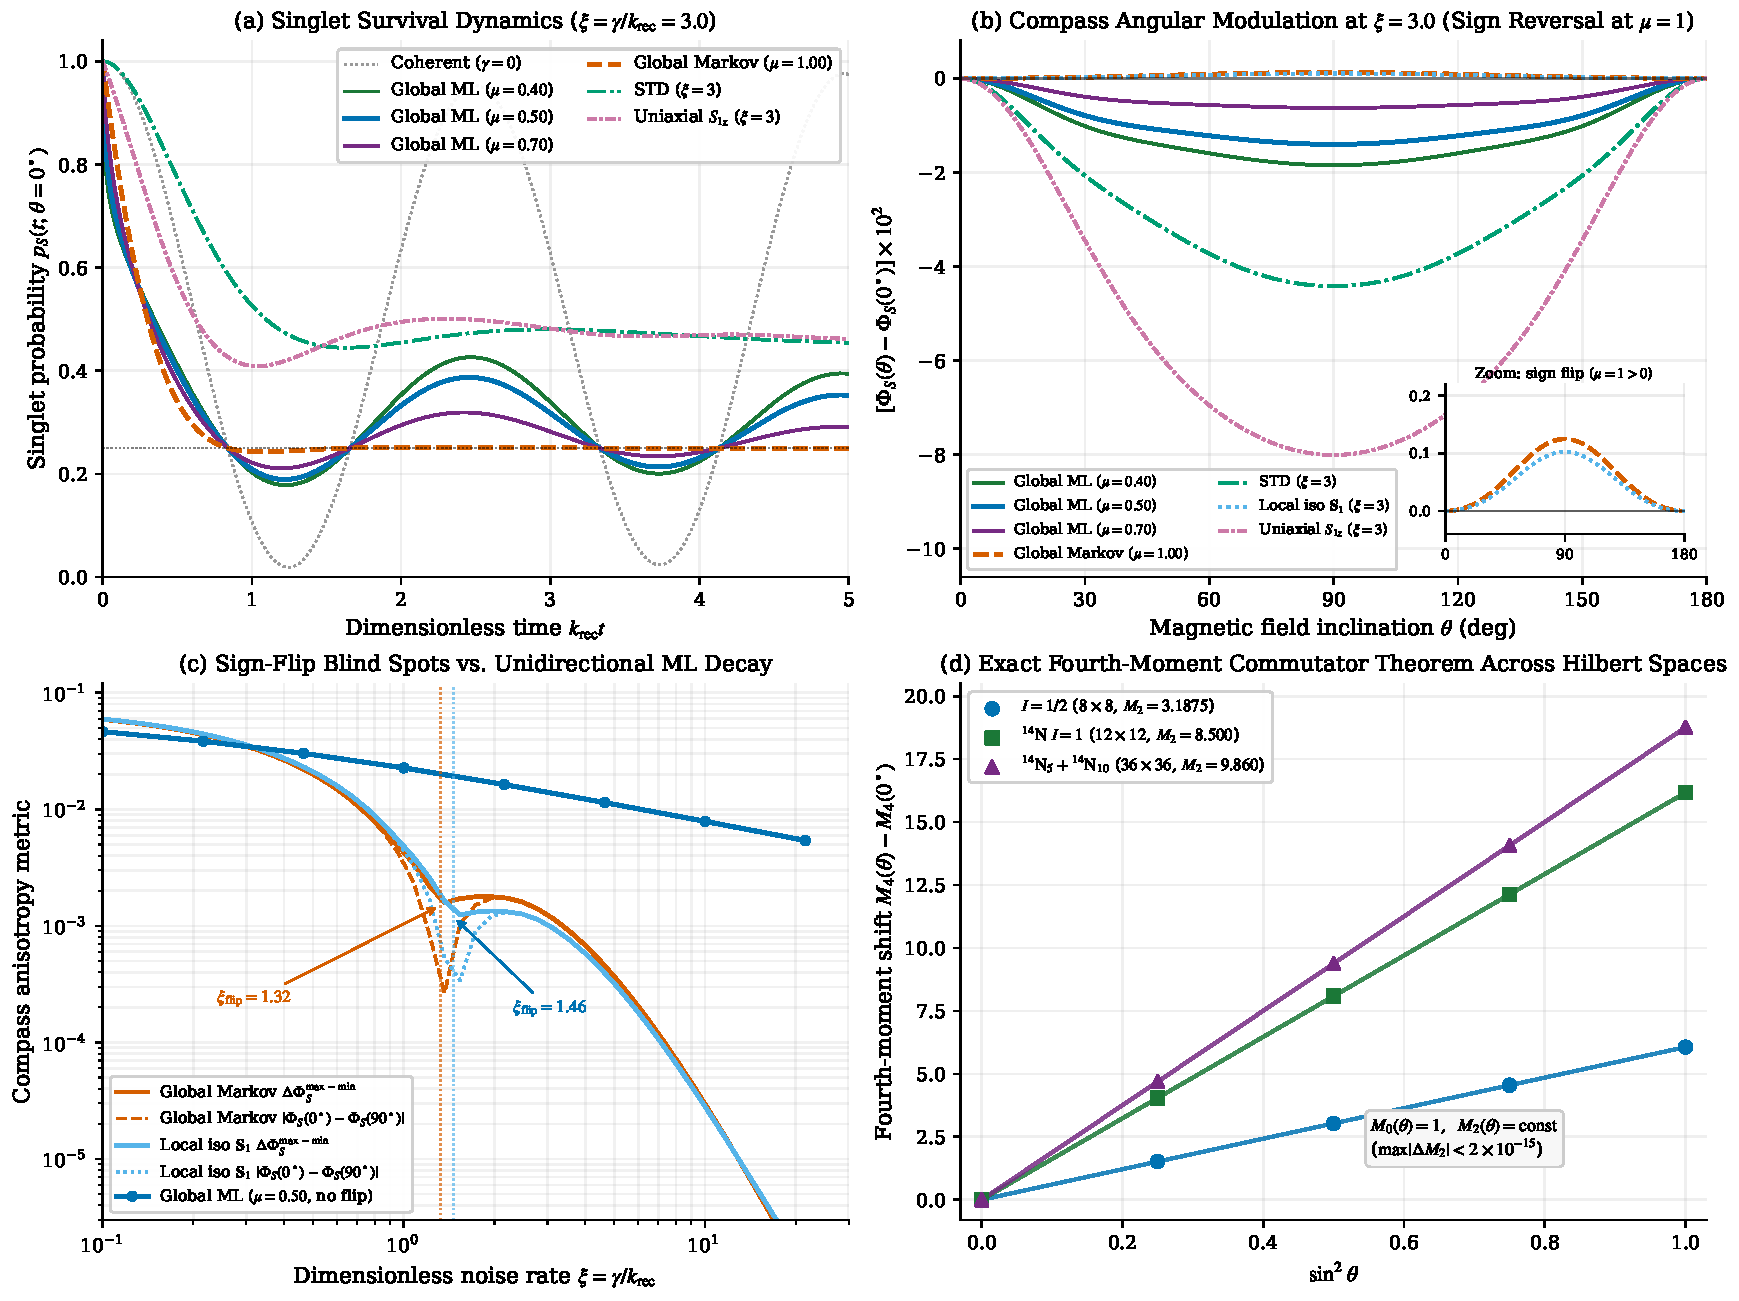
\includegraphics[width=\textwidth]{../figures/fig1_commutator_protection_and_blind_spot.pdf}
\caption{Fourth-Moment Commutator Protection and the Sign-Flip Blind Spot. \textbf{(a)} Singlet survival $p_S(t;\theta=0^\circ)$ at $\xi=3.0$ comparing coherent oscillations, global Mittag--Leffler ($\mu \in \{0.40,0.50,0.70\}$), global Markov ($\mu=1.00$), STD, and uniaxial $S_{1z}$ dynamics. \textbf{(b)} Angular modulation $\Phi_S(\theta)-\Phi_S(0^\circ)$ at $\xi=3.0$: global Markov and local isotropic $\mathbf{S}_1$ have flipped sign relative to $\mu < 1$, STD, and $S_{1z}$. \textbf{(c)} Signed $|\Phi_S(0^\circ)-\Phi_S(90^\circ)|$ vs.\ full angular span $\Delta\Phi_S^{\max-\min}$ in the canonical $8\times 8$ system: sign flips occur at $\xiflip = 1.3233$ (global Markov) and $\xiflip = 1.4599$ (local isotropic $\mathbf{S}_1$), where $\Delta\Phi_S^{\max-\min}$ retains only non-monotonic higher harmonics ($\approx 1.52\times 10^{-3}$ and $1.19\times 10^{-3}$), whereas $\mu=0.50$ ML decays monotonically without flipping. \textbf{(d)} Exact linear verification of Eq.~\eqref{eq:M4_axial} across $8\times 8$, $12\times 12$, and $36\times 36$ Hilbert spaces with $M_0=1$ and $\max|\Delta M_2| < 2\times 10^{-15}$.}
\label{fig1}
\end{figure*}

Figure~\ref{fig1}(b)--(c) demonstrates this reversal numerically: in the canonical $8\times 8$ model, global Markovian depolarization undergoes an exact sign flip at $\xiflip = 1.32330$ ($\Phi_S(0^\circ)-\Phi_S(90^\circ) = 2.78\times 10^{-16}$), and local isotropic $\mathbf{S}_1$ noise flips at $\xiflip = 1.45989$ ($-1.67\times 10^{-16}$). Even across the full $[0^\circ,180^\circ]$ interval, $\Delta\Phi_S^{\max-\min}$ drops to residual fourth-harmonic dips of $1.525\times 10^{-3}$ and $1.189\times 10^{-3}$, respectively, while in the physical $50\,\mu\text{T}$ $\mathrm{FAD}^{\bullet-}$ $36\times 36$ model, Brent root-finding locates the exact Markovian reversal at $\xiflip = 412.06$ (between $+9.860\times 10^{-8}$ at $\xi=300$ and $-1.579\times 10^{-9}$ at $\xi=1000$) and the local isotropic $\mathbf{S}_1$ reversal at $\xiflip = 685.02$.

\subsection{Mittag--Leffler \texorpdfstring{$\Theta(\xi^{5-\mu})$}{Theta(xi\^{}(5-mu))} Separation}

For completely monotonic Mittag--Leffler relaxation with $0 < \mu < 1$, Pollard's theorem~\cite{Pollard1948BAMS,Gorenflo2002FCAA} represents $E_\mu(-(\gamma t)^\mu)$ as a positive superposition of exponential rates $\int_0^\infty \ee^{-\gamma r t} K_\mu(r)\,\dd r$ with heavy spectral density $K_\mu(r) \sim [\pi\Gamma(1-\mu)]^{-1} r^{\mu-1}$ as $r \to 0^+$. Expanding Eq.~\eqref{eq:PhiS_ML_spectral} for $\gamma \gg |k+\ii\omega_{ab}|$ yields the leading asymptotic term directly:
\begin{align}
\label{eq:ML_asym}
\Phi_S^{(\mu)}(\theta) - \frac{1}{4} &= \xi^{-\mu}\,\Biggl[\sum_{a,b} W_{ab}(\theta) \operatorname{Re}\!\Bigl(\bigl(1 + \ii\tfrac{\omega_{ab}}{k}\bigr)^{\mu-1}\Bigr) - \frac{1}{4}\Biggr] \nonumber\\
&\quad + O(\xi^{-2\mu}),
\end{align}
using $k\frac{(k+\ii\omega)^{\mu-1}}{(k+\ii\omega)^\mu + \gamma^\mu} = \xi^{-\mu}(1+\ii\omega/k)^{\mu-1}[1 + O(\xi^{-\mu})]$. Because $f_{\mu}(\Omega) := \operatorname{Re}[(1+\ii\Omega)^{\mu-1}] = (1+\Omega^2)^{(\mu-1)/2}\cos\bigl((1-\mu)\arctan\Omega\bigr)$ is strictly positive and strictly decreasing near $\Omega \sim 1$ for $0<\mu<1$---avoiding the $\Omega^2$-protected cancellation of the Markovian Lorentzian---the leading directional coefficient $c_{\mathrm{ML}}(\theta) := \sum_{a,b} [W_{ab}(0) f_\mu(\omega_{ab}(0)/k) - W_{ab}(\theta) f_\mu(\omega_{ab}(\theta)/k)]$ is generically non-zero, giving $\DeltaPhi^{(\mu)} = c_{\mathrm{ML}}(\theta)\xi^{-\mu} + O(\xi^{-2\mu}) = \Theta(\xi^{-\mu})$. Whenever $c_{\mathrm{ML}}(\theta) \neq 0$ and $\Delta M_4(\theta) \neq 0$, comparing Eq.~\eqref{eq:ML_asym} with Theorem~\ref{thm:xi5_blindspot} gives
\begin{equation}
\label{eq:xi5minusmu}
\frac{|\DeltaPhi^{(\mu)}(\xi)|}{|\DeltaPhi^{(1)}(\xi)|} = \Theta\bigl(\xi^{5-\mu}\bigr) \qquad (0 < \mu < 1,\ \xi \gg 1).
\end{equation}
For $\mu = 0.50$, this yields $\Theta(\xi^{9/2}) = \Theta(t^9)$ when $\xi = t^2$; in $50\,\mu\text{T}$ $\mathrm{FAD}^{\bullet-}\text{--}\mathrm{Z}^{\bullet}$ (Table~\ref{tab:channels}), log--log exponents measure $\alpha = 0.3844$ ($\mu=0.40$), $0.4970$ ($\mu=0.50$), $0.7143$ ($\mu=0.70$), and $0.8714$ ($\mu=0.85$) over $\xi \in [10^2, 10^4]$ (converging tightly to $0.3916, 0.4994, 0.7051, 0.8550$ on $\xi \in [10^3, 10^4]$, and $0.5000$ on $[10^4, 10^6]$ for $\mu=0.50$), versus $\alpha = 4.9989$ on $[10^4, 10^6]$ for Markovian $\mu=1.00$ ($\alpha = 4.9986$ with tilted dipolar $d(r) = +50.0\,\text{rad}\,\mu\text{s}^{-1}$, $r=1.870\,\text{nm}$, matching $-\Delta M_4/(k^4\xi^5)$ to ratio $0.9999944$ at $\xi=10^6$). Moreover, in the canonical $8\times 8$ system no sign flips occur across $\xi \in [0.1, 31.6]$ for any $\mu \in \{0.40,0.50,0.70,0.85\}$ ($\min[\Phi_S(0^\circ)-\Phi_S(90^\circ)] = 2.39\times 10^{-4}$ at $\mu=0.85$, vs.\ $-1.75\times 10^{-3}$ at $\mu=1.00$).

%==============================================================================
\section{Five-Channel Liouvillian Taxonomy and Feshbach--Schur Dark Manifolds}
\label{sec:taxonomy}
%==============================================================================

While Eq.~\eqref{eq:xi5minusmu} governs global commuting relaxation, realistic spin relaxation operates via \emph{local} or \emph{partially commuting} Lindblad superoperators $\mathcal{L}_{\mathrm{tot}}(\theta) = -\ii[H_{\mathrm{RP}}(\theta),\cdot] - \frac{k_S}{2}\{P_S,\cdot\} - \frac{k_T}{2}\{P_T,\cdot\} + \gamma \mathcal{D}_{\mathrm{ch}}$~\cite{Worster2016JCP,Kattnig2016PCCP,Fay2018JCP}, where $\mathcal{D}[L](\rho) := L\rho L^\dagger - \frac{1}{2}\{L^\dagger L, \rho\}$ denotes the standard Lindblad dissipator and the resolvent singlet yield is
\begin{equation}
\label{eq:Liouville_yield}
\Phi_S(\theta) = k_S \Tr\!\bigl[\PS\,(-\mathcal{L}_{\mathrm{tot}}(\theta))^{-1}(\rho_0)\bigr], \qquad \rho_0 = \frac{\PS}{d_I}.
\end{equation}
Crucially, stopping numerical sweeps at $\xi \sim 10$ misidentifies asymptotic exponents because physical hyperfine frequencies ($A_\parallel = 5.0$ canonical, $309.38\,\mu\text{s}^{-1}$ in $\mathrm{FAD}^{\bullet-}$) have not yet entered $\gamma \gg \|\HRP\|$. Carrying native 45-digit \texttt{mpmath} superoperator solves out to $\xi \in [10^2, 10^4]$ (and $[10^4, 3{\times}10^6]$ at $50\,\mu\text{T}$) uncovers five distinct Feshbach--Schur dark-manifold scaling laws (Fig.~\ref{fig2}, Table~\ref{tab:channels}).

\begin{figure*}[t]
\centering
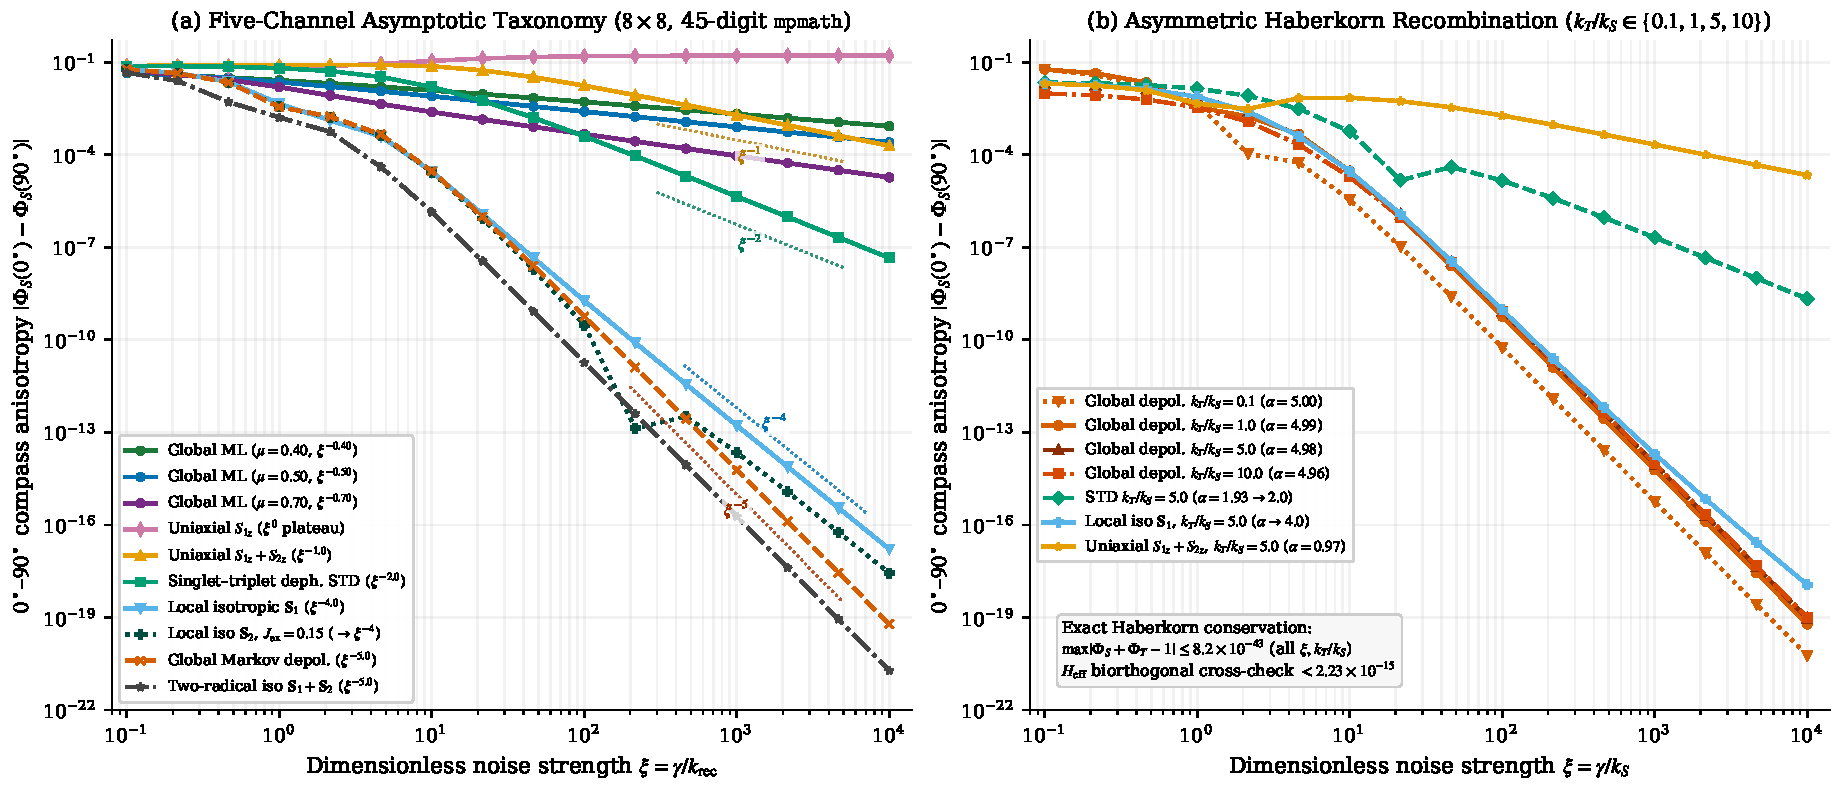
\includegraphics[width=\textwidth]{../figures/fig2_five_channel_taxonomy.pdf}
\caption{Five-channel asymptotic scaling taxonomy out to $\xi = 10^4$ in native 45-digit \texttt{mpmath} precision. \textbf{(a)} Symmetric $k_S = k_T = 1$ sweeps for the canonical $8\times 8$ system: global ML ($\xi^{-\mu}$), uniaxial $S_{1z}$ ($\xi^0$ plateau), uniaxial $S_{1z}+S_{2z}$ ($\xi^{-1.0}$), STD ($\xi^{-2.0}$), local isotropic $\mathbf{S}_1$ ($\xi^{-4.0}$), local isotropic $\mathbf{S}_2$ with $J_{\mathrm{ex}}=0.15$ undergoing a second sign reversal between $\xi=100$ and $215.4$ before locking onto $\xi^{-4}$ ($\alpha = 3.903$ on $[10^3,10^4]$, $3.966$ on $[4642,10^4]$), global Markov ($\xi^{-5.0}$), and two-radical isotropic $\mathbf{S}_1+\mathbf{S}_2$ ($\xi^{-5.0}$). \textbf{(b)} Asymmetric Haberkorn recombination ($k_T/k_S \in \{0.1,1,5,10\}$): exact trace preservation $\max|\Phi_S+\Phi_T-1| \le 8.2\times 10^{-43}$ and biorthogonal $H_{\mathrm{eff}}$ Sherman--Morrison cross-check error $< 2.23\times 10^{-15}$; every asymptotic power law ($\alpha \in \{5, 2, 4, 1\}$) persists cleanly.}
\label{fig2}
\end{figure*}

\subsection{Feshbach--Schur Dark-Manifold Derivation}

Decompose operator space $\mathcal{B}(\mathcal{H}) = \mathcal{M}_{\mathrm{dark}} \oplus \mathcal{M}_{\mathrm{bright}}$ according to $\mathcal{D}_{\mathrm{ch}}\!\mid_{\mathcal{M}_{\mathrm{dark}}} = 0$ and $-\mathcal{D}_{\mathrm{ch}}\!\mid_{\mathcal{M}_{\mathrm{bright}}} \ge c_0 > 0$. Writing $\mathcal{L}_{\mathrm{tot}} = \mathcal{L}_0 + \gamma\mathcal{D}_{\mathrm{ch}}$ where $\mathcal{L}_0 = -\ii\mathrm{ad}_{\HRP} - \frac{k_S}{2}\{\PS,\cdot\} - \frac{k_T}{2}\{\PT,\cdot\}$ and applying Feshbach--Schur projection $P_{\mathrm{D}}$ onto $\mathcal{M}_{\mathrm{dark}}$ ($Q_{\mathrm{B}} = \mathbb{I}-P_{\mathrm{D}}$) yields the exact dark-manifold effective superoperator:
\begin{align}
\label{eq:Schur}
\mathcal{L}_{\mathrm{eff}}(\theta) &= P_{\mathrm{D}}\mathcal{L}_0 P_{\mathrm{D}} \nonumber\\
&\quad - P_{\mathrm{D}}\mathcal{L}_0 Q_{\mathrm{B}}\bigl(Q_{\mathrm{B}}(\mathcal{L}_0 + \gamma\mathcal{D}_{\mathrm{ch}})Q_{\mathrm{B}}\bigr)^{-1} Q_{\mathrm{B}}\mathcal{L}_0 P_{\mathrm{D}}.
\end{align}
Tracking how $\theta$-dependent coherent operators ($\HZ$ and $\HHF$) couple $\mathcal{M}_{\mathrm{dark}}$ through $\mathcal{M}_{\mathrm{bright}}$ yields all five scaling classes:

\begin{enumerate}[leftmargin=1.4em,itemsep=2pt]
\item \textbf{Channel 1 --- Global Commuting Depolarization ($\mathcal{D}_{\mathrm{dep}}$):} Here $\mathcal{M}_{\mathrm{dark}} = \mathrm{span}\{\mathbb{I}\}$, decoupled from $\HRP$. All $\theta$-dependence traverses $\mathcal{M}_{\mathrm{bright}}$, where Theorem~\ref{thm:xi5_blindspot} enforces $\DeltaPhi = \Theta(\xi^{-5})$.
\item \textbf{Channel 2 --- Singlet--Triplet Dephasing ($\mathcal{D}_{\mathrm{STD}}(\rho) = \PS\rho\PS + \PT\rho\PT - \rho = \frac{1}{2}\mathcal{D}[\PS-\PT]$):} Here $\mathcal{M}_{\mathrm{dark}} = \PS\mathcal{B}(\mathcal{H})\PS \oplus \PT\mathcal{B}(\mathcal{H})\PT$ contains $\rho_0 = \PS/d_I$, while bright singlet--triplet coherences decay at rate $\gamma$ ($\mathcal{D}_{\mathrm{STD}}|_{Q_{\mathrm{B}}} = -\mathbb{I}_{Q_{\mathrm{B}}}$). In Eq.~\eqref{eq:Schur}, $P_{\mathrm{D}}\mathrm{ad}_{\HRP}Q_{\mathrm{B}} = P_{\mathrm{D}}\mathrm{ad}_{\HHF}Q_{\mathrm{B}}$ because $[\HZ,\PS]=[\Hex,\PS]=[\Hdip,\PS]=0$ leaves $\mathrm{ad}_{\HZ}$, $\mathrm{ad}_{\Hex}$, and $\mathrm{ad}_{\Hdip}$ block-diagonal within $\mathcal{M}_{\mathrm{dark}}$ and $\mathcal{M}_{\mathrm{bright}}$. Expanding $(Q_{\mathrm{B}}\mathcal{L}_0 Q_{\mathrm{B}} - \gamma\mathbb{I})^{-1} = -\gamma^{-1}\mathbb{I} - \gamma^{-2}Q_{\mathrm{B}}\mathcal{L}_0 Q_{\mathrm{B}} - \cdots$ yields $\mathcal{L}_{\mathrm{eff}} = L_{\mathrm{D}}(\theta) + \gamma^{-1} G_1 + \gamma^{-2} G_2 + O(\gamma^{-3})$, where $L_{\mathrm{D}}(\theta) := P_{\mathrm{D}}\mathcal{L}_0(\theta) P_{\mathrm{D}}$, $G_1 := P_{\mathrm{D}}\mathcal{L}_0 Q_{\mathrm{B}}\mathcal{L}_0 P_{\mathrm{D}}$ is $\theta$-independent, and $G_2 := P_{\mathrm{D}}\mathcal{L}_0 Q_{\mathrm{B}}\mathcal{L}_0 Q_{\mathrm{B}}\mathcal{L}_0 P_{\mathrm{D}}$. Expanding $k\Tr[\PS(-\mathcal{L}_{\mathrm{eff}})^{-1}\rho_0]$ for symmetric $k_S=k_T=k$ (where $(-L_{\mathrm{D}}(\theta))^{-1}\rho_0 = k^{-1}\rho_0$) shows that: (i) the $O(\gamma^{-1})$ Zeno leakage term $k^{-1}\gamma^{-1}\Tr[\PS G_1 \rho_0] = -M_2/(k\gamma)$ is strictly $\theta$-independent by Theorem~\ref{thm:M0M2}~\cite{Dellis2012Biosystems,Tiersch2012PhilTrans}; (ii) the $O(\gamma^{-2})$ bright-space trace $\Tr[\PS G_2 \rho_0] = k M_2$ is \emph{likewise} $\theta$-independent (because $\Tr(\PS[\HHF,[\HZ,[\HHF,\PS]]]) = 0$ by cyclicity and $[\HZ,\PS]=0$); and (iii) directional anisotropy first enters at $O(\gamma^{-2})$ through the \emph{dark-triplet iterate}
\begin{align}
\label{eq:STD_dark_iterate}
\DeltaPhi^{\mathrm{STD}} &= \frac{1}{k\gamma^2}\,\Delta_\theta\Tr\!\Bigl[\PS G_1 \bigl(-L_{\mathrm{D}}(\theta)\bigr)^{-1} G_1(\rho_0)\Bigr] \nonumber\\
&\quad + O(\gamma^{-3}),
\end{align}
in which $G_1(\rho_0)$ excites triplet-subspace populations/coherences inside $\PT\mathcal{B}(\mathcal{H})\PT$ that precess under the $\theta$-dependent dark Zeeman propagator $(-L_{\mathrm{D}}(\theta))^{-1}$ before returning to $\PS$. On the canonical $8\times 8$ system, Eq.~\eqref{eq:STD_dark_iterate} evaluates analytically to $+4.51208\,\xi^{-2}$, matching the exact 45-digit Liouvillian yield $+4.50600\,\xi^{-2}$ at $\xi=10^4$ to $0.13\%$ ($\alpha = 1.975$--$1.988$ in $8\times 8$, $1.912$ in $12\times 12$, $1.892$ canonical $36\times 36$; a rate-scaled reduced two-mode surrogate of this Zeno $M_2$-cancellation mechanism is formalized in Lean Theorem~\leanid{std\_zeno\_two\_sided\_xi2}).
\item \textbf{Channel 3 --- Local Isotropic Spin Noise ($\mathcal{D}_{\mathrm{iso},1} = \sum_\alpha \mathcal{D}[S_{1\alpha}]$ vs.\ $\mathcal{D}_{\mathrm{iso},2}$ vs.\ $\mathcal{D}_{\mathrm{iso},12}$):} Because isotropic spin-$1/2$ depolarization on electron~1 annihilates every traceless $S_{1\alpha}$ operator at eigenvalue $-1$ ($\mathcal{D}_{\mathrm{iso},1}|_{Q_{\mathrm{B}}} = -\mathbb{I}_{Q_{\mathrm{B}}}$), its dark manifold is $\mathcal{M}_{\mathrm{dark}} = \mathbb{I}_2^{(1)} \otimes \mathcal{B}(\mathcal{H}_2 \otimes \mathcal{H}_{\mathrm{nuc}})$. Crucially, $\rho_0 - \mathbb{I}/D = -\frac{1}{d_I}\mathbf{S}_1\cdot\mathbf{S}_2$ lies strictly inside $\mathcal{M}_{\mathrm{bright}}$, and a single action of $\mathcal{L}_0$ cannot reach $\mathcal{M}_{\mathrm{dark}}$: $P_{\mathrm{D}}\mathcal{L}_0 Q_{\mathrm{B}}\rho_0 = 0$ identically (and symmetrically $(Q_{\mathrm{B}}\PS)^\dagger \mathcal{L}_0 P_{\mathrm{D}} = 0$), because $\mathrm{ad}_{\HZ}$, $\mathrm{ad}_{\Hex}$, $\mathrm{ad}_{\Hdip}$, and $\mathrm{ad}_{\HHF}$ acting once on $\mathbf{S}_1\cdot\mathbf{S}_2$ produce only operators traceless on electron~1 (via $[S_{1\alpha}, S_{1\beta}] = \ii\epsilon_{\alpha\beta\gamma}S_{1\gamma}$). Entering $\mathcal{M}_{\mathrm{dark}}$ therefore requires \emph{two} bright steps: $P_{\mathrm{D}}\mathcal{L}_0 Q_{\mathrm{B}}\mathcal{L}_0 Q_{\mathrm{B}}\rho_0 \neq 0$, generated by $S_{1\alpha}S_{1\alpha'} = \frac{1}{4}\delta_{\alpha\alpha'}\mathbb{I}_2^{(1)} + \frac{\ii}{2}\epsilon_{\alpha\alpha'\gamma}S_{1\gamma}$ together with non-commuting nuclear operators $[I_\beta, I_{\beta'}] \neq 0$ (producing dark operators $\propto \mathbb{I}_2^{(1)} \otimes S_{2\alpha}[I_\beta,I_{\beta'}]$ at order $\gamma^{-2}$). Inside $\mathcal{M}_{\mathrm{dark}}$, electron~2 precesses freely at $O(\gamma^0)$ under the $\theta$-dependent dark propagator $(-P_{\mathrm{D}}\mathcal{L}_0(\theta)P_{\mathrm{D}})^{-1}$, and returning to $Q_{\mathrm{B}}\PS$ requires two additional bright steps (another factor $\gamma^{-2}$). Combining all four bright propagators gives the exact leading four-bright-step Feshbach--Schur cascade
\begin{align}
\label{eq:iso1_fourstep}
\DeltaPhi^{\mathrm{iso},1} &= \frac{k}{\gamma^4}\,\Delta_\theta\Bigl\langle Q_{\mathrm{B}}\PS,\; \mathcal{L}_0 Q_{\mathrm{B}}\mathcal{L}_0 P_{\mathrm{D}} \bigl(-L_{\mathrm{D}}(\theta)\bigr)^{-1} \nonumber\\
&\quad \times P_{\mathrm{D}}\mathcal{L}_0 Q_{\mathrm{B}}\mathcal{L}_0 Q_{\mathrm{B}}\rho_0 \Bigr\rangle + O(\gamma^{-5}) = \Theta(\xi^{-4}).
\end{align}
On the canonical $8\times 8$ system, Eq.~\eqref{eq:iso1_fourstep} evaluates analytically to $-0.163885\,\xi^{-4}$, agreeing to $0.13\%$ with the exact 45-digit Liouvillian result $-0.164100\,\xi^{-4}$ at $\xi = 10^4$ ($\alpha = 4.0234$ on $\xi \in [10^2, 10^4]$, converging to $\alpha_{\mathrm{loc}} = 4.00032$ at $\xi \approx 4.3\times 10^4$; a reduced rational-block surrogate exhibiting $\Theta(\xi^{-4})$ scaling is formalized in Lean Theorem~\leanid{local\_iso\_dark\_xi4}). Conversely, if $\mathcal{D}_{\mathrm{iso},2}$ acts solely on the hyperfine-free electron~2 ($e_k = 1\;\forall k$), then when $J_{\mathrm{ex}}=0$ and $\Hdip = 0$ no coupling connects $\mathcal{M}_{\mathrm{dark}} = \mathcal{B}(\mathcal{H}_1\otimes\mathcal{H}_{\mathrm{nuc}})\otimes\mathbb{I}_2^{(2)}$ to $\mathbf{S}_1\cdot\mathbf{S}_2$ at any order, restoring $\Theta(\xi^{-5})$ ($\alpha = 4.9902$). Turning on $J_{\mathrm{ex}} = 0.15$ re-opens the four-step bridge through $\mathcal{M}_{\mathrm{dark}}$, triggering a second sign reversal between $\xi=100$ ($-3.01\times 10^{-10}$) and $\xi=215.4$ ($+1.36\times 10^{-13}$) after which the post-reversal slope locks cleanly onto $\Theta(\xi^{-4})$ ($\alpha = 3.9032$ on $[10^3, 10^4]$, reaching $3.9238 \to 3.9661$ on consecutive intervals, Fig.~\ref{fig2}(a)). When both radicals undergo independent isotropic relaxation ($\mathcal{D}_{\mathrm{iso},12}$), $\mathcal{M}_{\mathrm{dark}}$ shrinks to $\mathcal{B}(\mathcal{H}_{\mathrm{nuc}})$, restoring $\Theta(\xi^{-5})$ ($\alpha = 4.9952$).
\item \textbf{Channel 4 --- Local Uniaxial Spin Dephasing ($\mathcal{D}_{z,12}$ vs.\ $\mathcal{D}_{z,1}$):} Two-electron uniaxial dephasing $\mathcal{D}_{z,12} = \mathcal{D}[S_{1z}] + \mathcal{D}[S_{2z}]$ kills all electronic $x,y$ components while preserving the Ising correlation $S_{1z} S_{2z}$ (which overlaps $\PS$) inside $\mathcal{M}_{\mathrm{dark}}$. When $\theta = 0^\circ$ ($\hat{\mathbf{b}} = \hat{\mathbf{z}}$), $[\HZ(0), S_{1z} S_{2z}] = 0$ leaves the Ising dark state decoupled from bright $x,y$ modes, whereas for $\theta \neq 0^\circ$, transverse Zeeman field $\omega_L \sin\theta (S_{1x} + S_{2x})$ leaks directly out of $S_{1z}S_{2z}$ into the $\gamma$-damped bright manifold at Schur rate $v^2/\gamma = \Theta(\xi^{-1})$, yielding $\DeltaPhi = \Theta(\xi^{-1})$ (reduced block in Lean Theorem~\leanid{local\_z\_leak\_xi1}; $\alpha = 0.9773$ in $8\times 8$, $0.9719$ in $12\times 12$, $0.9749$ canonical $36\times 36$). Rotating the dephasing axis to $\mathcal{D}_{x,12}$ mirrors this at $\theta=90^\circ$ ($\alpha = 0.8963$ trending toward $1.0$). Conversely, \emph{single-electron} uniaxial noise $\mathcal{D}_{z,1}$ in a reference-probe radical pair ($e_k = 1\;\forall k$, $\Hdip = 0$, $k_S = k_T = k$) leaves $\mathbf{S}_2$ untouched inside the $S_{1z}=\pm 1/2$ diagonal manifold $\mathcal{M}_{\mathrm{dark}} = \mathrm{span}\{\mathbb{I}_2^{(1)}, S_{1z}\}\otimes\mathcal{B}(\mathcal{H}_2\otimes\mathcal{H}_{\mathrm{nuc}})$, where $\mathbf{S}_2$ precesses freely at $O(\xi^0)$ under $\omega_L\hat{\mathbf{b}}\cdot\mathbf{S}_2 \mp J_{\mathrm{ex}} S_{2z}$, producing a strictly non-decaying $\Theta(\xi^0)$ plateau (reduced $J_{\mathrm{ex}}=0$ single-mode block in Lean Theorem~\leanid{local\_z\_single\_sat\_xi0}):
\begin{equation}
\label{eq:local_z1_sat}
\Delta\Phi_{S,\infty}^{\mathcal{D}_{z,1}} := \lim_{\xi\to\infty}\bigl[\Phi_S(0^\circ) - \Phi_S(90^\circ)\bigr] = \frac{\omega_L^2}{4(k^2 + \omega_L^2 + J_{\mathrm{ex}}^2)}.
\end{equation}
For canonical parameters ($\omega_L=1.40, J_{\mathrm{ex}}=0.15, k=1.0$), Eq.~\eqref{eq:local_z1_sat} gives $0.164292$, matching $0.164209$ ($8\times 8$) and $0.164198$ ($12\times 12$) at $\xi=10^4$; for physical $50\,\mu\text{T}$ $\mathrm{FAD}^{\bullet-}\text{--}\mathrm{Z}^{\bullet}$ ($\omega_L=8.804298, J_{\mathrm{ex}}=0$), it predicts $0.246816$, matching $0.246652$ at $\xi=10^6$.
\item \textbf{Channel 5 --- Asymmetric Haberkorn Recombination ($k_S \neq k_T$):} Writing the anti-commutator decay as $-\ii(H_{\mathrm{eff}}\rho - \rho H_{\mathrm{eff}}^\dagger)$ with $H_{\mathrm{eff}} = \HRP - \ii\frac{k_S}{2}\PS - \ii\frac{k_T}{2}\PT$~\cite{Haberkorn1976MolPhys,Fay2018JCP}, we verified across $k_T/k_S \in \{0.1, 1.0, 5.0, 10.0\}$ using native 45-digit split-operator assembly both exact total yield conservation ($\max|\Phi_S+\Phi_T-1| \le 8.2\times 10^{-43}$ across all 17 channel sweeps) and agreement to $< 2.23\times 10^{-15}$ against an independent biorthogonal Sherman--Morrison rank-1 eigen-solver. As Table~\ref{tab:channels} and Fig.~\ref{fig2}(b) show, $k_T \neq k_S$ modulates prefactors (scaling as $\frac{16 k_S k_T^2}{(k_S+3k_T)^2}$ under global depolarization, vanishing if $k_T \to 0$ when $\Phi_S \to 1$) and crossover locations (e.g.\ iso-$\mathbf{S}_1$ at $k_T/k_S=5$ displays $\alpha = 4.4566 \to 4.0$), because asymmetric decay mixes $\PS$ and $\PT$ inside $\mathcal{L}_0$ only at $O(\gamma^0)$, leaving every strong-noise scaling class ($\alpha \in \{5, 2, 4, 1\}$) intact for all $k_S, k_T > 0$.
\end{enumerate}

\begin{table*}[t]
\centering
\caption{Five-channel asymptotic scaling exponents $\alpha = -\dd\ln|\DeltaPhi|/\dd\ln\xi$ fitted over $\xi \in [10^2, 10^4]$. Entries marked $\dagger$ denote physical $50\,\mu\text{T}$ $\mathrm{FAD}^{\bullet-}\text{--}\mathrm{Z}^{\bullet}$ extended-tail slopes past the hyperfine crossover ($[10^4, 10^6]$ for global ML/Markov; $[10^5, 10^6]$ for sparse local/STD channels, where final-interval slopes reach $1.5392$ on $[3{\times}10^5, 10^6]$ for STD, $0.9969$ for $S_{1z}+S_{2z}$, and $3.9853$ on $[10^6, 3{\times}10^6]$ for $\mathbf{S}_1$); $\ddagger$ denotes the $8\times 8$ local slope at $\xi \approx 4.3{\times}10^4$; ``can.'' denotes canonical $36\times 36$ parameters ($12\times 12$ gives $4.9868$ for global Markov). Parentheses for local uniaxial $S_{1z}$ report the saturated plateau $\DeltaPhi$ at $\xi_{\max}$. Adding $35^\circ$-tilted dipolar coupling ($d(r)=+50.0\,\text{rad}\,\mu\text{s}^{-1}$, $D_{\mathrm{ZFS}}=-75.0\,\text{rad}\,\mu\text{s}^{-1}$, $r=1.870\,\text{nm}$) to $50\,\mu\text{T}$ $\mathrm{FAD}^{\bullet-}\text{--}\mathrm{Z}^{\bullet}$ preserves global Markov $\alpha = 4.9986^\dagger$.}
\label{tab:channels}
\setlength{\tabcolsep}{3.5pt}
\resizebox{\textwidth}{!}{%
\begin{tabular}{@{}llccccc@{}}
\toprule
Channel & Superoperator & Theory & $8{\times}8$ ($k_T{=}k_S$) & $8{\times}8$ ($k_T{=}5k_S$) & $36{\times}36$ can. & $36{\times}36$ $50\,\mu\text{T}$ \\
\midrule
Global ML ($\mu=0.40$) & $E_{0.40}(-(\gamma t)^{0.40})$ & $0.40$ & $0.3940$ & --- & --- & $0.3844$ \\
Global ML ($\mu=0.50$) & $E_{0.50}(-(\gamma t)^{0.50})$ & $0.50$ & $0.4999$ & --- & $0.4994$ & $0.4970$ ($0.5000^\dagger$) \\
Global ML ($\mu=0.70$) & $E_{0.70}(-(\gamma t)^{0.70})$ & $0.70$ & $0.7015$ & --- & --- & $0.7143$ \\
Global ML ($\mu=0.85$) & $E_{0.85}(-(\gamma t)^{0.85})$ & $0.85$ & $0.8499$ & --- & --- & $0.8714$ \\
\midrule
Global Markov ($\mu=1$) & $\mathcal{D}_{\mathrm{dep}}$ & $5$ & $4.9902$ & $4.9782$ & $4.9881$ ($12{\times}$: $4.9868$) & $4.9989^\dagger$ ($4.9986^\dagger$ dip.) \\
Global Markov ($k_T/k_S$) & $\mathcal{D}_{\mathrm{dep}}$ & $5$ & \multicolumn{2}{c}{$4.9953$ ($k_T{=}0.1$) / $4.9646$ ($k_T{=}10$)} & --- & --- \\
Singlet--triplet (STD) & $\frac{1}{2}\mathcal{D}[\PS-\PT]$ & $2$ & $1.9754$ & $1.9277$ & $1.8923$ & $0.4088 \to 1.3056^\dagger$ \\
STD (full norm) & $\mathcal{D}[\PS-\PT]$ & $2$ & $1.9875$ & --- & --- & --- \\
Local isotropic $\mathbf{S}_1$ & $\sum_\alpha \mathcal{D}[S_{1\alpha}]$ & $4$ & $4.0234$ ($4.0003^\ddagger$) & $4.4566$ & $4.0331$ & $2.5989 \to 3.9151^\dagger$ \\
Local isotropic $\mathbf{S}_2$ ($J{=}0.15$) & $\sum_\alpha \mathcal{D}[S_{2\alpha}]$ & $5\to 4$ & $3.9032^{\S}$ ($3.9661$ tail) & --- & --- & --- \\
Local isotropic $\mathbf{S}_2$ ($J{=}0$) & $\sum_\alpha \mathcal{D}[S_{2\alpha}]$ & $5$ & $4.9902$ & --- & --- & --- \\
Local isotropic $\mathbf{S}_1{+}\mathbf{S}_2$ & $\mathcal{D}_{\mathrm{iso},1}+\mathcal{D}_{\mathrm{iso},2}$ & $5$ & $4.9952$ & --- & --- & --- \\
Local uniaxial $\mathbf{S}_1{+}\mathbf{S}_2$ ($z$) & $\mathcal{D}[S_{1z}]+\mathcal{D}[S_{2z}]$ & $1$ & $0.9773$ & $0.9717$ & $0.9749$ & $0.5333 \to 0.9939^\dagger$ \\
Local uniaxial $\mathbf{S}_1{+}\mathbf{S}_2$ ($x$) & $\mathcal{D}[S_{1x}]+\mathcal{D}[S_{2x}]$ & $1$ & $0.8963$ & --- & --- & --- \\
Local uniaxial $S_{1z}$ & $\mathcal{D}[S_{1z}]$ & $0$ & $-0.0093$ ($0.1642$) & --- & $-0.0109$ ($0.1642$) & $-0.0026^\dagger$ ($0.2467$) \\
\bottomrule
\multicolumn{7}{@{}l@{}}{\scriptsize $^{\S}$Undergoes a second sign reversal between $\xi=100$ and $215.4$; post-reversal slope fitted over $[10^3,10^4]$ ($3.9238 \to 3.9661$ on consecutive intervals).}
\end{tabular}%
}
\end{table*}

%==============================================================================
\section{\texorpdfstring{Microscopic Non-Commuting Colored-Bath Crucible: Prony ADO, Single-Mode OU, and $50\,\mu\text{T}$ $\mathrm{FAD}^{\bullet-}$}{Microscopic Non-Commuting Colored-Bath Crucible: Prony ADO, Single-Mode OU, and 50 uT FAD.-}}
\label{sec:ado}
%==============================================================================

\subsection{Separating Phenomenological Memory from Local Spin Baths}

Because $\mathcal{D}_{\mathrm{dep}}$ acts globally and commutes with $\HRP$, Eq.~\eqref{eq:xi5minusmu} must \emph{never} be interpreted as claiming that biological cryptochrome obeys global commuting Mittag--Leffler relaxation. Physical protein environments subject radical-pair electrons to \emph{local, non-commuting} stochastic magnetic fields $\delta\mathbf{B}(t)$ coupled via $H_{\mathrm{noise}}(t) = \sum_{\alpha} \delta B_\alpha(t) S_{1\alpha}$~\cite{Kattnig2016PCCP,Worster2016JCP,Fay2019JCP} with colored autocorrelation
\begin{align}
\label{eq:C_powerlaw}
C(t) &= \sigma^2 \left(1 + \frac{|t|}{\tau_c}\right)^{-\mu}, \nonumber\\
\int_0^{u_{\max}\tau_c} \frac{C(t)}{\sigma^2}\,\dd t &= \tau_c\,\frac{(1+u_{\max})^{1-\mu}-1}{1-\mu},
\end{align}
parameterized independently by the RMS field amplitude $\sigma$ ($\mu\text{s}^{-1}$), the short-time ultraviolet (UV) correlation time $\tau_c$ ($\mu\text{s}$), and the power-law exponent $\mu \in (0,1)$, alongside two axis geometries: \emph{3D isotropic} fields ($\alpha \in \{x,y,z\}$ independently) and \emph{uniaxial} $z$-fields ($\alpha = z$ only). For $0 < \mu < 1$, the bare power-law integral diverges on $[0,\infty)$, so Eq.~\eqref{eq:C_powerlaw} requires a long-time infrared (IR) cutoff $u_{\max} = t_{\max}/\tau_c \gg 1$ (giving $61.28\,\tau_c$ at $\mu=0.50, u_{\max}=10^3$).

To solve non-Markovian local colored baths beyond Redfield theory~\cite{Fay2019JCP,Tanimura2020JCP}, we perform non-negative least-squares (NNLS) plus variable-projection Prony fitting~\cite{Tanimura1989JPSJ,Tanimura2020JCP} of $(1 + u)^{-\mu} \approx \sum_{m=1}^K \tilde{c}_m \ee^{-\tilde{\nu}_m u}$ over dimensionless lag $u = t/\tau_c \in [0, 10^3]$. Choosing $K=8$ strictly positive exponentials guarantees positivity ($\tilde{c}_m, \tilde{\nu}_m > 0$) and achieves maximum relative errors of $0.0248\%$ ($\mu=0.40$), $0.0363\%$ ($\mu=0.50$), $0.226\%$ ($\mu=0.70$), and $0.694\%$ ($\mu=0.85$) across four decades of $u$ (Fig.~\ref{fig3}(a)). Setting $c_m = \sigma^2 \tilde{c}_m$ and $\nu_m = \tilde{\nu}_m / \tau_c$ defines the IR-regularized integrated correlation time of the Prony surrogate,
\begin{equation}
\label{eq:tau_int_prony}
\tau_{\mathrm{int}} := \int_0^\infty \frac{C_{\mathrm{Prony}}(t)}{\sigma^2}\,\dd t = \tau_c \sum_{m=1}^K \frac{\tilde{c}_m}{\tilde{\nu}_m},
\end{equation}
yielding $\tau_{\mathrm{int}} = 138.399\,\tau_c$ ($\mu=0.50$) and $15.263\,\tau_c$ ($\mu=0.85$), dominated by the slowest Prony mode ($\tilde{\nu}_8 = 3.981\times 10^{-4}$ for $\mu=0.50$, i.e.\ effective IR cutoff $u_{\mathrm{IR}} = 1/\tilde{\nu}_8 = 2512$). In the fast-bath motional-narrowing limit $\sigma\tau_{\mathrm{int}} \ll 1$, second-order cumulant expansion yields the rate-matched Markovian relaxation rate $\gamma_{\mathrm{eff}} = 2\sigma^2 \tau_{\mathrm{int}}$ entering $\mathcal{L}_{\mathrm{Markov}} = \mathcal{L}_0 + \gamma_{\mathrm{eff}}\mathcal{D}_{\mathrm{ch}}$ ($\mathcal{D}_{\mathrm{ch}} \in \{\mathcal{D}_{\mathrm{iso},1}, \mathcal{D}_{z,1}\}$). Crucially, we also benchmark every $1/f^\alpha$ ensemble directly against a \emph{single-mode Ornstein--Uhlenbeck bath} (OU1), $C_{\mathrm{OU1}}(t) = \sigma^2 \ee^{-t/\tau_{\mathrm{int}}}$, carrying the exact same RMS amplitude $\sigma$ and exact same integrated correlation time $\tau_{\mathrm{int}}$ (hence identical zero-frequency spectral density $S(0) = 2\sigma^2\tau_{\mathrm{int}}$).

Mapping Eq.~\eqref{eq:tau_int_prony} into a deterministic Tanimura--Kubo Auxiliary Density Operator (ADO) hierarchy~\cite{Ishizaki2005JPSJ,Tanimura2020JCP} (audited over $N_{\mathrm{ADO}} \in [200, 2500]$, converging to $<10^{-4}$), we cross-check independently against antithetic/cubic-paired OU--MC ensembles of $900$--$1400$ trajectories ($1200$--$1400$ for 3D isotropic baths, $900$ for uniaxial $z$, $\Delta t_{\mathrm{eff}} \le 0.008\,\mu\text{s}$). At $(\tau_c = 0.005, \sigma = 1.5, \mu = 0.50)$, 3D isotropic ADO ($N_{\mathrm{ADO}}=2500$) gives $\DeltaPhi = 0.041054$ versus OU--MC $0.04036 \pm 0.00083$ ($0.83\sigma$); across Protocol~A ($\tau_c = 0.001, 0.003$, $N_{\mathrm{ADO}}=1800$), 3D ADO and OU--MC agree identically within statistical error bars ($0.02619$ vs.\ $0.02617 \pm 0.00119$ at $\tau_c=0.001$; $0.01764$ vs.\ $0.01828 \pm 0.00124$ at $\tau_c=0.003$).

\begin{figure*}[t]
\centering
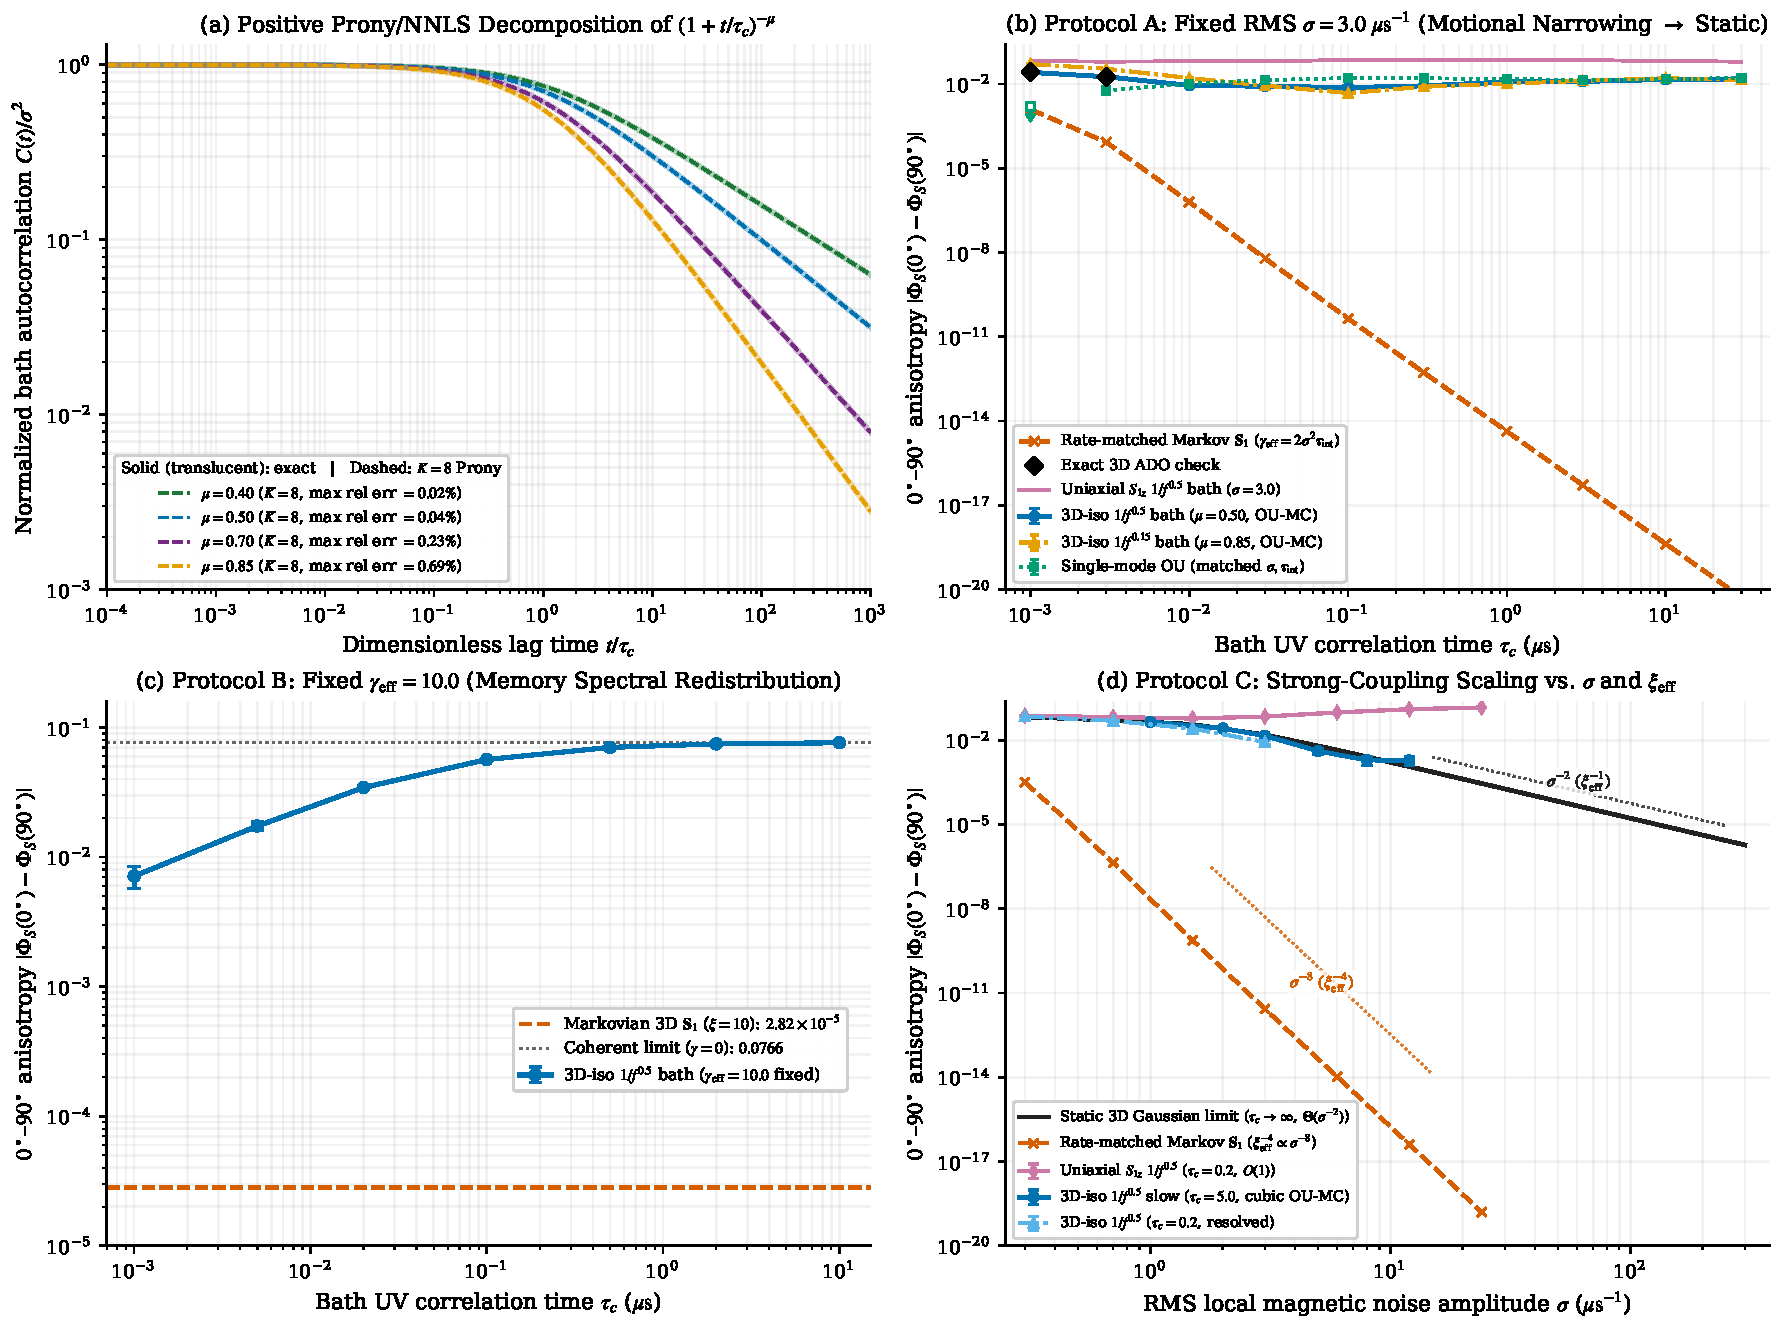
\includegraphics[width=\textwidth]{../figures/fig3_microscopic_ado_crucible.pdf}
\caption{Microscopic non-commuting $1/f^\alpha$ spin-bath crucible in the canonical $8\times 8$ system. \textbf{(a)} Positive $K=8$ Prony/NNLS approximations to $C(t)/\sigma^2 = (1+t/\tau_c)^{-\mu}$ over $t/\tau_c \in [10^{-4}, 10^3]$ ($\le 0.69\%$ max rel.\ error). \textbf{(b)} Protocol~A (fixed RMS $\sigma=3.0\,\mu\text{s}^{-1}$, $\tau_c \in [10^{-3}, 30]\,\mu\text{s}$): extrapolating rate-matched Markovian 3D isotropic depolarization ($\gamma_{\mathrm{eff}}=2\sigma^2\tau_{\mathrm{int}}$) beyond motional narrowing collapses $\DeltaPhi$ as $\tau_c^{-4}$, whereas bounded-RMS 3D-$1/f^{0.5}$ ($\mu=0.50$), 3D-$1/f^{0.15}$ ($\mu=0.85$), and matched single-mode OU1 baths all saturate onto the quasi-static plateau ($\approx 0.015\text{--}0.017$) at large $\tau_c$---while diverging sharply at short $\tau_c = 0.001\text{--}0.003\,\mu\text{s}$ where multi-timescale $1/f^{0.5}$ outperforms resonant single-mode OU1 (confirmed deterministically by exact 3D ADO, black diamonds). Uniaxial $S_{1z}$ remains $O(1)$. \textbf{(c)} Protocol~B (fixed $\gamma_{\mathrm{eff}} = 10.0\,\mu\text{s}^{-1}$, $\sigma \propto \tau_c^{-1/2}$): increasing $\tau_c$ lowers $\sigma$ and shifts power away from $\omega_L, A_\parallel$, lifting 3D isotropic anisotropy from $+0.00712$ toward the coherent limit ($0.07664$). \textbf{(d)} Protocol~C ($\sigma$-sweep at fixed $\tau_c=0.2, 5.0\,\mu\text{s}$): colored 3D noise transitions from Markovian $\sigma^{-8}$ ($\xi_{\mathrm{eff}}^{-4}$) toward the $\sigma^{-2}$ static 3D Gaussian limit ($\alpha_\sigma = 1.996$, with $\tau_c=5.0$ slow OU--MC reaching $\alpha_\sigma = 1.945$ over $\sigma \in [2,8]\,\mu\text{s}^{-1}$).}
\label{fig3}
\end{figure*}

\subsection{Three Diagnostic Protocols: Motional-Narrowing Breakdown and \texorpdfstring{$1/f^\alpha$}{1/f\^{}alpha} vs.\ Single-Mode OU}

Testing non-commuting $1/f^\alpha$ magnetic noise across three diagnostic protocols (Table~\ref{tab:ado}, Fig.~\ref{fig3}) isolates the exact physics cleanly without conflating Redfield breakdown with anomalous memory:

\begin{enumerate}[leftmargin=1.4em,itemsep=2pt]
\item \textbf{Protocol~A --- Fixed RMS $\sigma = 3.0\,\mu\text{s}^{-1}$, Increasing Memory $\tau_c \in [0.001, 30]\,\mu\text{s}$:} Rate-matching a Markovian Lindblad model via $\gamma_{\mathrm{eff}} = 2\sigma^2\tau_{\mathrm{int}} \propto \tau_c$ sweeps $\xi_{\mathrm{eff}}$ from $2.49$ to $74{,}735$. Extrapolating this second-order fast-bath formula past $\sigma\tau_c \gtrsim 1$ fails catastrophically, driving 45-digit Markovian 3D isotropic anisotropy down as $\xi_{\mathrm{eff}}^{-4}$ from $-1.258\times 10^{-3}$ ($\tau_c=0.001$) to $-5.254\times 10^{-21}$ ($\tau_c=30.0$). Even in the physically legitimate intermediate regime $\tau_c = 0.001\text{--}0.003\,\mu\text{s}$ ($\gamma_{\mathrm{eff}} = 2.49\text{--}7.47\,\mu\text{s}^{-1}$), Markovian Lindblad already underestimates the exact 3D-$1/f^{0.5}$ ADO contrast by $20.8\times$ to $207.7\times$ and mispredicts its sign. Crucially, comparing $1/f^{0.5}$ against the \emph{matched single-mode OU1 bath} at identical $(\sigma, \tau_{\mathrm{int}})$ exposes where broadband $1/f^\alpha$ structure genuinely matters versus where it does not:
  \begin{itemize}[leftmargin=1.2em,itemsep=1pt]
  \item \emph{Short-$\tau_c$ resonant crossover ($\tau_c = 0.001\text{--}0.003\,\mu\text{s}$):} Single-mode OU1 concentrates 100\% of its variance $\sigma^2$ at a single rate $1/\tau_{\mathrm{int}} \approx 7.23\,\mu\text{s}^{-1}$ right near the canonical hyperfine scale $A_\parallel = 5.0$, crushing contrast to $+0.00006 \pm 0.00151$ ($\tau_c=0.001$) and $+0.00592 \pm 0.00141$ ($\tau_c=0.003$). By contrast, $1/f^{0.5}$ spreads $\sigma^2$ across four decades of rates---shifting substantial weight into ultra-fast motionally narrowed modes ($\nu_m \gg A_\parallel$) and ultra-slow quasi-static modes ($\nu_m \ll k_{\mathrm{rec}}$)---retaining $+0.02619$ ($>17\sigma$ above OU1) and $+0.01764$ ($>6\sigma$ above OU1).
  \item \emph{Intermediate crossover ($\tau_c = 0.1\,\mu\text{s}$):} The relation inverts: OU1's single pole has already dropped below $k_{\mathrm{rec}}$ ($1/\tau_{\mathrm{int}} = 0.072\,\mu\text{s}^{-1}$, entering the static plateau early at $+0.01649 \pm 0.00113$), whereas $1/f^{0.5}$ retains residual fast modes near $\omega_L, A_\parallel$ that still dephase the pair ($+0.00751 \pm 0.00150$).
  \item \emph{Quasi-static slow-bath limit ($\tau_c \ge 3.0\,\mu\text{s}$):} Once all bath modes freeze below $k_{\mathrm{rec}}$, $1/f^{0.5}$ ($+0.01526 \pm 0.00093$), $1/f^{0.15}$ ($+0.01399 \pm 0.00100$), and single-mode OU1 ($+0.01672 \pm 0.00099$) converge to the same static inhomogeneous-broadening plateau determined by $\sigma < A_\parallel$, proving that long-$\tau_c$ preservation is a generic consequence of bounded-RMS escape from motional narrowing rather than a unique signature of $1/f^\alpha$ tails.
  \end{itemize}
Under uniaxial $S_{1z}$ colored noise, $\DeltaPhi$ sits stably across $+0.063$--$0.075$ for all $\tau_c \in [0.001, 30]\,\mu\text{s}$, consistent with its $O(\xi^0)$ dark manifold.
\item \textbf{Protocol~B --- Fixed Zero-Frequency Spectral Density $\gamma_{\mathrm{eff}} = 2\sigma^2\tau_{\mathrm{int}} = 10.0\,\mu\text{s}^{-1}$:} Holding $S(0) = \gamma_{\mathrm{eff}}$ fixed while increasing $\tau_c \in [0.001, 10.0]\,\mu\text{s}$ simultaneously reduces the RMS field amplitude as $\sigma = (\gamma_{\mathrm{eff}} / 2\tau_{\mathrm{int}})^{1/2} \propto \tau_c^{-1/2} \to 0$ ($6.011 \to 0.060\,\mu\text{s}^{-1}$) and narrows the bath bandwidth below $\omega_L, A_\parallel$. Consequently, 3D-$1/f^{0.5}$ anisotropy rises monotonically from $+0.00712 \pm 0.00139$ ($\tau_c=0.001$, $253\times$ over Markovian $-2.816\times 10^{-5}$) to $+0.07621 \pm 0.00002$ ($\tau_c=10.0$, $2706\times$ over Markovian, recovering $99.4\%$ of the coherent limit $0.07664$).
\item \textbf{Protocol~C (Strong-Coupling Static Crossover vs.\ $\sigma$):} Sweeping $\sigma$ at fixed $\tau_c$ tests strong-noise scaling directly in the physical RMS field. Rate-matched Markovian 3D depolarization drops as $\gamma_{\mathrm{eff}}^{-4} \propto \sigma^{-8}$, whereas numerical integration of an exact static 3D Gaussian field ensemble ($\tau_c \to \infty$) establishes $\DeltaPhi^{\mathrm{static}} \propto \sigma^{-2}$ ($\alpha_\sigma = 1.9962$ at high $\sigma$). In 400-seed OU--MC at $\tau_c = 5.0\,\mu\text{s}$, the resolved power law reaches $\sigma^{-1.9445}$ (i.e.\ $\xi_{\mathrm{eff}}^{-0.9722}$) across $\sigma \in [2, 8]\,\mu\text{s}^{-1}$ (matching the static $\sigma^{-2}$ law within statistical uncertainty; extending to $\sigma=12\,\mu\text{s}^{-1}$ near the $\sim 7\times 10^{-4}$ MC variance floor gives $\alpha_\sigma = 1.5978$ over $[2,12]$), outlasting $\sigma^{-8}$ because quasi-static fields leave field-aligned spin components unscrambled within the radical lifetime.
\end{enumerate}

\begin{table*}[t]
\centering
\caption{Microscopic non-commuting 3D isotropic $1/f^{0.5}$ ($\mu=0.50$) vs.\ matched single-mode OU1 (identical $\sigma,\tau_{\mathrm{int}}$) and rate-matched Markovian $\mathcal{D}_{\mathrm{iso},1}$ across Protocols A and B in the canonical $8\times 8$ system. Uncertainties are $1\sigma$ standard errors over $1200$--$1400$ OU--MC trajectories; 45-digit \texttt{mpmath} resolves $\Delta\Phi_{S,\mathrm{Markov}}$ beyond float64 precision at large $\gamma_{\mathrm{eff}}$.}
\label{tab:ado}
\setlength{\tabcolsep}{4pt}
\renewcommand{\arraystretch}{0.93}
\resizebox{\textwidth}{!}{%
\begin{tabular}{@{}lccccccc@{}}
\toprule
Protocol & $\tau_c$ ($\mu$s) & $\sigma$ ($\mu\text{s}^{-1}$) & $\gamma_{\mathrm{eff}}$ ($\mu\text{s}^{-1}$) & $\Delta\Phi_{S,\mathrm{Markov}}$ & $\Delta\Phi_{S,\mathrm{ADO}}$ ($1/f^{0.5}$) & $\Delta\Phi_{S,\mathrm{OU-MC}}$ ($1/f^{0.5}$) & $\Delta\Phi_{S,\mathrm{OU1}}$ (matched) \\
\midrule
Prot.\ A & $0.001$ & $3.000$ & $2.491$ & $-1.258\times 10^{-3}$ & $+0.02619$ & $+0.02617(119)$ & $+0.00006(151)$ \\
Prot.\ A & $0.003$ & $3.000$ & $7.474$ & $-8.490\times 10^{-5}$ & $+0.01764$ & $+0.01828(124)$ & $+0.00592(141)$ \\
Prot.\ A & $0.100$ & $3.000$ & $249.1$ & $-4.480\times 10^{-11}$ & --- & $+0.00751(150)$ & $+0.01649(113)$ \\
Prot.\ A & $3.000$ & $3.000$ & $7473.5$ & $-5.263\times 10^{-17}$ & --- & $+0.01244(118)$ & $+0.01402(91)$ \\
Prot.\ A & $30.00$ & $3.000$ & $74735.3$ & $-5.254\times 10^{-21}$ & --- & $+0.01526(93)$ & $+0.01672(99)$ \\
\midrule
Prot.\ B & $0.001$ & $6.011$ & $10.0$ & $-2.816\times 10^{-5}$ & --- & $+0.00712(139)$ & --- \\
Prot.\ B & $0.100$ & $0.601$ & $10.0$ & $-2.816\times 10^{-5}$ & --- & $+0.05657(61)$ & --- \\
Prot.\ B & $10.00$ & $0.060$ & $10.0$ & $-2.816\times 10^{-5}$ & --- & $+0.07621(2)$ & --- \\
\bottomrule
\end{tabular}%
}
\end{table*}

\subsection{Non-Commuting Colored-Bath Dynamics in Physical \texorpdfstring{$50\,\mu\text{T}$ $36\times 36$ $\mathrm{FAD}^{\bullet-}$}{50 uT 36x36 FAD.-}}

To confirm that these local colored-bath conclusions transfer directly to realistic geomagnetic cryptochrome scales rather than only toy $8\times 8$ parameters, we propagated BLAS-batched exact integrated-OU SU(2) Strang-split ensembles directly on the full $36\times 36$ $^{14}\text{N}_5 + {}^{14}\text{N}_{10}$ $\mathrm{FAD}^{\bullet-}\text{--}\mathrm{Z}^{\bullet}$ Hamiltonian at $B_0 = 50\,\mu\text{T}$ ($\omega_L = 8.804\,\text{rad}\,\mu\text{s}^{-1}$, $k_{\mathrm{rec}} = 1.0\,\mu\text{s}^{-1}$, coherent baseline $\DeltaPhi^{\mathrm{coh}} = +0.20729$) under 3D isotropic local magnetic noise on $\mathbf{S}_1$ with $\sigma = 5.0\,\text{rad}\,\mu\text{s}^{-1}$ ($\approx 28.4\,\mu\text{T}$ RMS local field) across $\tau_c \in [0.001, 10.0]\,\mu\text{s}$ ($N_{\mathrm{traj}} = 200$ paired trajectories per angle, $\Delta t = 0.001\,\mu\text{s}$, $T_{\max} = 12.0\,\mu\text{s}$ so $\ee^{-k_{\mathrm{rec}}T_{\max}} = 6.1\times 10^{-6}$). Exact sampling of the joint Gaussian $(\eta(t+\Delta t), \Delta t^{-1}\!\int_t^{t+\Delta t}\eta(s)\,\dd s)$ preserves exact variance even for fast Prony modes with $\nu_m \Delta t > 1$; an independent step-halving check at the stiffest point ($\tau_c = 0.001\,\mu\text{s}$, $\Delta t = 0.0005\,\mu\text{s}$) yields $+0.19441 \pm 0.00132$, matching $+0.19461 \pm 0.00141$ at $\Delta t = 0.001\,\mu\text{s}$ to $0.10\%$ ($0.10\sigma$).

Table~\ref{tab:fad_colored} reveals three clean physical signatures:
(i) Even at nanosecond UV correlation time $\tau_c = 1\,\text{ns}$ ($0.001\,\mu\text{s}$, $\gamma_{\mathrm{eff}} = 6.92\,\mu\text{s}^{-1}$), where rate-matched Markovian isotropic relaxation already degrades the $50\,\mu\text{T}$ compass by more than an order of magnitude ($\DeltaPhi = +0.01517$), the exact non-Markovian $1/f^{0.5}$ bath preserves $+0.19461 \pm 0.00141$ ($93.9\%$ of the noiseless coherent contrast, $12.8\times$ above Markovian);
(ii) at $\tau_c = 0.001\text{--}0.01\,\mu\text{s}$, $1/f^{0.5}$ yields slightly \emph{lower} contrast ($> 5\sigma$) than matched single-mode OU1 ($+0.20431 \pm 0.00104$ and $+0.20790 \pm 0.00104$) because the large $^{14}\text{N}_5$ hyperfine frequency ($A_{\mathrm{N5},\parallel} = 309\,\mu\text{s}^{-1}$) already places OU1's single pole ($1/\tau_{\mathrm{int}} = 7.23\,\mu\text{s}^{-1} \ll A_{\mathrm{N5},\parallel}$) in the quasi-static regime, whereas the high-frequency wing of $1/f^{0.5}$ still overlaps the hyperfine transitions;
(iii) for $\tau_c \ge 0.1\,\mu\text{s}$, the rate-matched Markovian channel crosses its blind spot ($\xiflip = 685.02$ for $\mathcal{D}_{\mathrm{iso},1}$) and flips sign to $-7.11\times 10^{-10} \to -1.16\times 10^{-13}$ (resolved via native 45-digit iterative refinement), while both $1/f^{0.5}$ and OU1 saturate cleanly at the coherent-scale inhomogeneous plateau $+0.205\text{--}0.207$.

\begin{table*}[t]
\centering
\caption{Direct non-commuting 3D isotropic colored-bath exact integrated-OU Monte Carlo simulations ($\Delta t = 0.001\,\mu\text{s}$, $T_{\max}=12.0\,\mu\text{s}$, $N_{\mathrm{traj}}=200$ paired trajectories) on the physical $50\,\mu\text{T}$ $36\times 36$ $^{14}\text{N}_5 + {}^{14}\text{N}_{10}$ $\mathrm{FAD}^{\bullet-}\text{--}\mathrm{Z}^{\bullet}$ radical pair ($\omega_L = 8.804\,\text{rad}\,\mu\text{s}^{-1}$, $k_{\mathrm{rec}}=1.0\,\mu\text{s}^{-1}$, $\sigma = 5.0\,\text{rad}\,\mu\text{s}^{-1}$, coherent baseline $\DeltaPhi^{\mathrm{coh}} = +0.20729$). Both $1/f^{0.5}$ and matched single-mode OU1 share identical $(\sigma, \tau_{\mathrm{int}} = 138.40\,\tau_c)$ and $\gamma_{\mathrm{eff}} = 2\sigma^2\tau_{\mathrm{int}}$; Markovian $\mathcal{D}_{\mathrm{iso},1}$ values are resolved by native 45-digit sparse iterative refinement. Step-halving at $\tau_c = 0.001\,\mu\text{s}$ ($\Delta t = 0.0005\,\mu\text{s}$) gives $+0.19441(132)$.}
\label{tab:fad_colored}
\setlength{\tabcolsep}{5pt}
\resizebox{\textwidth}{!}{%
\begin{tabular}{@{}cccccc@{}}
\toprule
$\tau_c$ ($\mu$s) & $\tau_{\mathrm{int}}$ ($\mu$s) & $\gamma_{\mathrm{eff}}$ ($\mu\text{s}^{-1}$) & $\Delta\Phi_{S,\mathrm{Markov}}$ ($\mathcal{D}_{\mathrm{iso},1}$) & $\Delta\Phi_{S,1/f^{0.5}}$ (OU--MC) & $\Delta\Phi_{S,\mathrm{OU1}}$ (matched) \\
\midrule
$0.001$ & $0.1384$ & $6.920$ & $+1.517\times 10^{-2}$ & $+0.19461(141)$ & $+0.20431(104)$ \\
$0.010$ & $1.3840$ & $69.20$ & $+7.461\times 10^{-5}$ & $+0.19763(113)$ & $+0.20790(104)$ \\
$0.100$ & $13.840$ & $692.0$ & $-7.109\times 10^{-10}$ & $+0.20440(106)$ & $+0.20751(104)$ \\
$1.000$ & $138.40$ & $6920$ & $-2.855\times 10^{-10}$ & $+0.20543(102)$ & $+0.20652(109)$ \\
$10.00$ & $1384.0$ & $69199$ & $-1.163\times 10^{-13}$ & $+0.20737(111)$ & $+0.20704(97)$ \\
\bottomrule
\end{tabular}%
}
\end{table*}

%==============================================================================
\section{Pre-Asymptotic Crossovers in Multi-Nucleus \texorpdfstring{$36\times 36$ $\mathrm{FAD}^{\bullet-}$}{36x36 FAD.-}}
\label{sec:fad}
%==============================================================================

\begin{figure*}[t]
\centering
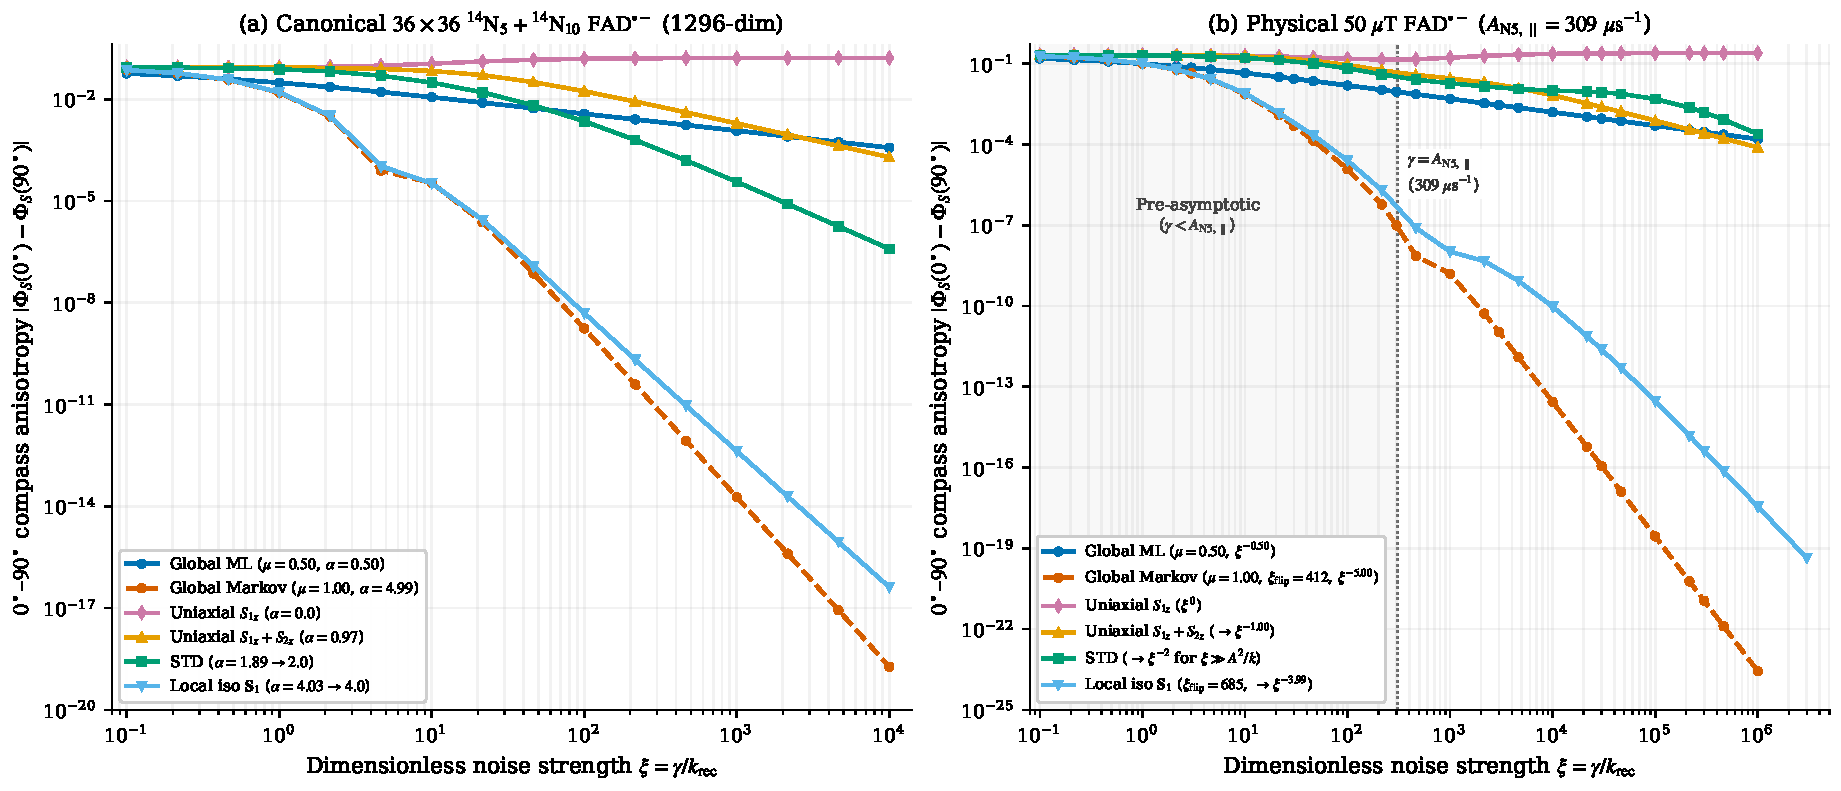
\includegraphics[width=0.96\textwidth]{../figures/fig4_realistic_fad_36x36.pdf}
\caption{Multi-nucleus $36\times 36$ ($1296$-dimensional Liouville) $^{14}\text{N}_5 + {}^{14}\text{N}_{10}$ $\mathrm{FAD}^{\bullet-}$ verification. \textbf{(a)} Canonical parameters ($\omega_L=1.40, A_{\mathrm{N5},\parallel}=5.0$) already enter all five asymptotic power laws ($\xi^{-0.50}$, $\alpha_{\mathrm{M}} = 4.99$, $\xi^0$, $\alpha_{z,12}=0.97$, $\alpha_{\mathrm{STD}}=1.89$, $\alpha_{\mathrm{iso},1}=4.03$) by $\xi = 10^2\text{--}10^4$. \textbf{(b)} Physical $B_0 = 50\,\mu\text{T}$ cryptochrome parameters ($A_{\mathrm{N5},\parallel} = 309.38\,\mu\text{s}^{-1}$, $k_{\mathrm{rec}} = 1\,\mu\text{s}^{-1}$): below $\gamma = A_{\mathrm{N5},\parallel}$ ($\xi \lesssim 309$), every local Markov channel sits in a pre-asymptotic crossover ($\alpha_{\mathrm{STD}} = 0.409$, $\alpha_{\mathrm{iso},1} = 2.599$, $\alpha_{z,12}=0.533$ over $\xi \in [10^2,10^4]$); exact blind spots lie at $\xiflip = 412.06$ (global Markov) and $\xiflip = 685.02$ (local isotropic $\mathbf{S}_1$). Extending to $\xi \in [10^4, 3{\times}10^6]$ recovers true $\alpha_{\mathrm{M}} = 4.999$, $\alpha_{\mathrm{iso},1} = 3.915$ ($[10^5,10^6]$) $\to 3.985$ ($[10^6,3{\times}10^6]$), $\alpha_{\mathrm{STD}} = 1.306 \to 1.539$ ($[3{\times}10^5,10^6]$), $\alpha_{z,12} = 0.994 \to 0.997$, and $\Delta\Phi_S^{z,1} \to 0.2467$.}
\label{fig4}
\end{figure*}

Figure~\ref{fig4} highlights why asymptotic claims for realistic cryptochrome require sweeping past the physical hyperfine scale. For physical $50\,\mu\text{T}$ $\mathrm{FAD}^{\bullet-}$~\cite{Lee2014JRSocInterface,Hore2016ARB} ($A_{\mathrm{N5},\parallel} = 309.38\,\mu\text{s}^{-1}$, $A_{\mathrm{N10},\parallel} = 106.88\,\mu\text{s}^{-1}$), the dimensionless scale $\gamma/A_\parallel$ shifts upward by nearly two orders of magnitude: $\gamma = A_{\mathrm{N5},\parallel}$ occurs only at $\xi \approx 309$, exact blind spots shift to $\xiflip = 412.06$ (global Markov) and $685.02$ (local iso-$\mathbf{S}_1$), and for STD the crossover $\gamma \sim A_{\mathrm{N5},\parallel}^2/k_{\mathrm{rec}} \approx 9.57\times 10^4$ pushes asymptotic $\xi^{-2}$ behavior beyond $\xi = 10^5$. Before $\xi=10^4$, all local channels exhibit gentler pre-asymptotic slopes ($\alpha_{\mathrm{STD}} = 0.4088$, $\alpha_{z,12}=0.5333$, $\alpha_{\mathrm{iso},1}=2.5989$ across $\xi \in [10^2,10^4]$). Extended sweeps to $\xi = 10^6$--$3{\times}10^6$ verify monotonic convergence onto the exact Feshbach--Schur laws: global Markov hits $\alpha = 4.9989$ across $[10^4, 10^6]$ ($-2.76\times 10^{-24}$ at $10^6$, and $\alpha = 4.9986$ with $35^\circ$-tilted dipolar $d(r)=+50.0\,\text{rad}\,\mu\text{s}^{-1}$, $r=1.870\,\text{nm}$); local isotropic $\mathbf{S}_1$ marches monotonically through consecutive intervals $[10^4,3{\times}10^4]$ ($3.3328$), $[3{\times}10^4,10^5]$ ($3.6738$), $[10^5,3{\times}10^5]$ ($3.8704$), $[3{\times}10^5,10^6]$ ($3.9547$, giving $3.9151$ across $[10^5,10^6]$), and $[10^6,3{\times}10^6]$ ($3.9853$, reaching $-4.438\times 10^{-20}$); uniaxial $S_{1z}+S_{2z}$ reaches $0.9939$ ($0.9969$ on $[3{\times}10^5, 10^6]$); $S_{1z}$ saturates at $0.24665$ ($\alpha = -0.0026 \to -0.0013$); and STD accelerates toward $2.0$ ($1.3056$ on $[10^5,10^6]$ and $1.5392$ on $[3{\times}10^5,10^6]$, reaching $0.9679$ singlet yield as Zeno freezing sets in).

%==============================================================================
\section{Machine-Checked Pure Lean~4 Formal Verification}
\label{sec:lean}
%==============================================================================

To eliminate subtle sign, projector-normalization, trace-cancellation, dipolar-orthogonality, or asymptotic-remainder errors, we formalized the core algebraic and analytical theorems in pure Lean~4.16.0 (\leanid{Paper1\_RadicalPair.lean}, 5,991 lines, zero Mathlib dependencies, zero \texttt{sorry}/\texttt{admit}, zero custom axioms, and zero \texttt{native\_decide}). The module constructs Gaussian rational arithmetic (\leanid{ZGauss}, \leanid{Q}, \leanid{CQ}), finite Kronecker block algebra (\leanid{finKron}, \leanid{MatCQ}), explicit $8\times 8$, $12\times 12$, and $36\times 36$ embeddings, an arbitrary-$K$-nucleus inductive tensor tower (\leanid{MultiNucSpec}, \leanid{MultiRP}) supporting arbitrary nuclear attachment $e\colon\mathrm{Fin}\,K\to\mathrm{Bool}$ ($e_k \in \{1,2\}$) and arbitrary symmetric electron--electron dipolar tensors $\mathbf{D}^\top = \mathbf{D}$ (\leanid{H\_dip}, \leanid{H\_RP\_gen\_dip}), and an ordered-field positive-power interface (\leanid{PosPowModel}). Concrete nuclear spin matrices are instantiated directly for $I=1/2$ and $I=1$, while higher nuclear spins $I \ge 3/2$ are covered via the abstract \leanid{MultiNucSpec} trace-weight axioms.

To maintain complete mathematical transparency, Table~\ref{tab:lean} distinguishes three levels of formalization scope:
\begin{itemize}[leftmargin=1.4em,itemsep=0.5pt,topsep=2pt,parsep=0pt]
\item \textbf{Full matrix and spectral proofs from first principles:} Every projector identity, commutator vanishing ($[\HZ,\PS]=[\Hex,\PS]=[\Hdip,\PS]=0$), $M_0/M_2/M_4$ invariance and anisotropy theorem across $4m\times 4m$, arbitrary $K$-nucleus models ($e_k \in \{1,2\}$, arbitrary symmetric $\mathbf{D}^\top=\mathbf{D}$), $36\times 36$ $\mathrm{FAD}^{\bullet-}$ corollaries, the Lorentzian resolvent identity~\eqref{eq:lorentz_exp}, the two-sided $\Theta(\xi^{-5})$ Markov envelope~\eqref{eq:xi5_bounds}, and the sign-flip guarantee and concrete witness are proved directly from explicit matrix and spectral definitions (while the bridge equating matrix traces $M_{2n}$ with spectral weights $\sum_{a,b} W_{ab}\omega_{ab}^{2n}$ via Hermitian diagonalization is analytic).
\item \textbf{Algebraic ratio bounds conditioned on analytic Mittag--Leffler estimates:} \leanid{ml\_half\_vs\_markov\_xi9\_2} and \leanid{ml\_separation\_general} formally certify the algebraic $\Omega(\xi^{5-\mu})$ separation against Theorem~\ref{thm:xi5_blindspot} given the analytic $\Omega(\xi^{-\mu})$ lower bound of Eq.~\eqref{eq:ML_asym}.
\item \textbf{Reduced Feshbach--Schur dark-manifold block bounds:} \leanid{schur\_complement\_2x2}, \leanid{std\_zeno\_two\_sided\_xi2}, \leanid{local\_iso\_dark\_xi4}, \leanid{local\_z\_leak\_xi1}, and \leanid{local\_z\_single\_sat\_xi0} certify exact two-sided rational scaling bounds on reduced $2\times 2$ and scalar rational-block Schur surrogates modeling the scaling mechanisms of Sec.~\ref{sec:taxonomy} (whereas the full $D^2$-dimensional dark-iterate formulas~\eqref{eq:STD_dark_iterate}--\eqref{eq:iso1_fourstep} are established analytically and verified numerically in 45-digit \texttt{mpmath}).
\end{itemize}
Source and kernel inspection confirms 364 authored public theorems (501 authored total including 137 private helpers) and 560 kernel-audited public \texttt{thmInfo} declarations (including all 69 headline theorems across \leanid{UnifiedRP} [28], \leanid{SymDip4} [3], \leanid{MultiRP} [23], and \leanid{StrongNoiseAsymptotics4C} [15]), with zero disallowed axioms beyond Lean's standard logical foundations (\leanid{propext}, \leanid{Quot.sound}, and \leanid{Classical.choice}).

\begin{table*}[t]
\centering
\caption{Selected machine-checked theorems in \leanid{Paper1\_RadicalPair.lean} (Lean~4.16.0, pure \texttt{Init}, 5,991 lines; 364 authored public theorems, 501 authored total, 560 kernel-audited public \texttt{thmInfo} entries including 69 headline main-section theorems, zero disallowed axioms). Axiom profile \textbf{PQ} denotes \texttt{[propext, Quot.sound]} and \textbf{PCQ} denotes \texttt{[propext, Classical.choice, Quot.sound]}.}
\label{tab:lean}
\setlength{\tabcolsep}{4pt}
\renewcommand{\arraystretch}{0.93}
\resizebox{\textwidth}{!}{%
\begin{tabular}{@{}llllc@{}}
\toprule
Theorem Identifier & Scope / Dim. & Mathematical Content Verified & Proof Scope & Axioms \\
\midrule
\leanid{PS\_idem}, \leanid{PS\_PT\_ortho}, \leanid{PS\_trace} & $4m \times 4m$ (\leanid{UnifiedRP}) & $\PS^2=\PS$, $\PS\PT=0$, $\Tr(\PS)=m$ & Full matrix & \textbf{PCQ}/\textbf{PQ} \\
\leanid{comm\_H\_Z\_PS}, \leanid{comm\_H\_ex\_PS} & $4m \times 4m$ (\leanid{UnifiedRP}) & $[\HZ(\hat{\mathbf{b}}),\PS]=0$, $[\Hex,\PS]=0$ & Full matrix & \textbf{PCQ} \\
\leanid{SymDip4\_eq\_half\_sum}, \leanid{comm\_SymDip4\_PS4}, \leanid{v4\_orthog\_SymDip4} & $4\times 4$ electron space & $[\mathrm{SymDip}_4(a,b),\PS]=0$ and $[\mathrm{SymDip}_4(a,b), V_c] \perp V_d$ & Full matrix & \textbf{PCQ} \\
\leanid{M0\_norm\_one}, \leanid{M2\_norm\_exact}, \leanid{M4\_diff\_unified} & $4m \times 4m$ (\leanid{UnifiedRP}) & $M_0=1$, exact $M_2$, Zeeman--hyperfine $\perp$, Eq.~\eqref{eq:M4_multi} ($K=1$) & Full matrix & \textbf{PCQ} \\
\leanid{M2\_8\_canonical}, \leanid{M4\_8\_axial\_diff}, \leanid{M4\_12\_axial\_diff}, \leanid{M4\_8\_canonical\_90deg} & $8\times 8$, $12\times 12$ explicit & $\frac{1}{8}$ ($I=1/2$) and $\frac{1}{3}$ ($I=1$) axial laws; $M_2=\frac{51}{16}$, $\Delta M_4=\frac{4851}{800}$ & Full matrix & \textbf{PCQ} \\
\leanid{MultiRP.M2\_multi\_gen}, \leanid{M4\_multi\_diff\_gen} & $K$ nuclei ($e_k\in\{1,2\}$) & Arbitrary multi-nucleus attachment Eqs.~\eqref{eq:M2_exact}--\eqref{eq:M4_multi} & Full matrix & \textbf{PCQ} \\
\leanid{MultiRP.H\_dip\_eq\_sym}, \leanid{comm\_H\_dip\_PS\_multi} & $K$ nuclei ($\mathbf{D}^\top=\mathbf{D}$) & Raw $\mathbf{S}_1\cdot\mathbf{D}\cdot\mathbf{S}_2$ commutes with $\PS$ & Full matrix & \textbf{PCQ} \\
\leanid{MultiRP.M2\_multi\_gen\_dip}, \leanid{M4\_multi\_diff\_gen\_dip} & $K$ nuclei ($e_k\in\{1,2\}, \mathbf{D}^\top=\mathbf{D}$) & Exact $M_2$ and $\Delta M_4$ invariance under arbitrary $J_{\mathrm{ex}}$ and $\mathbf{D}$ & Full matrix & \textbf{PCQ} \\
\leanid{MultiRP.FAD\_36x36\_twoN14\_dipolar\_M4\_diff} & $36\times 36$ ($\mathrm{FAD}^{\bullet-}$ + $\mathbf{D}$) & Exact $\frac{1}{3}\omega_L^2\sum_{k=1}^2$ law with arbitrary $e_k$ and symmetric $\mathbf{D}$ & Full matrix & \textbf{PCQ} \\
\leanid{lorentz\_resolvent\_identity}, \leanid{laplacePS\_expansion} & Finite spectral modes & Resolvent identity~\eqref{eq:lorentz_exp} and $s^{-1},s^{-3},s^{-5}$ expansion & Full spectral & \textbf{PQ} \\
\leanid{markov\_xi5\_envelope}, \leanid{markov\_sign\_flip\_guarantee}, \leanid{sign\_flip\_blind\_spot\_witness} & General mode spectra & Strict two-sided $\Theta(\xi^{-5})$ bounds~\eqref{eq:xi5_bounds} + reversal witness & Full spectral & \textbf{PQ} \\
\leanid{ml\_half\_vs\_markov\_xi9\_2}, \leanid{ml\_separation\_general} & $\mathbb{Q}$; \leanid{PosPowModel} & $\Omega(t^9)$ ($\mu=\frac{1}{2}$) and general $\Omega(\xi^{5-\mu})$ vs.\ Markov $\xi^{-5}$ & Alg.\ ratio (cond.) & \textbf{PQ} \\
\leanid{schur\_complement\_2x2}, \leanid{std\_zeno\_two\_sided\_xi2} & Reduced $2{\times}2$ blocks & Feshbach--Schur identity~\eqref{eq:Schur} and STD $M_2$ Zeno $\Theta(\xi^{-2})$ & Reduced Schur & \textbf{PQ} \\
\leanid{local\_iso\_dark\_xi4}, \leanid{local\_z\_leak\_xi1}, \leanid{local\_z\_single\_sat\_xi0} & Reduced dark blocks & $\Theta(\xi^{-4})$ (iso $\mathbf{S}_1$), $\Theta(\xi^{-1})$ ($S_{1z}+S_{2z}$), $\Theta(\xi^0)$ ($S_{1z}$, $J_{\mathrm{ex}}=0$ block) & Reduced Schur & \textbf{PQ} \\
\bottomrule
\end{tabular}%
}
\end{table*}

%==============================================================================
\section{Discussion, Physical Caveats, and Conclusions}
\label{sec:conclusions}
%==============================================================================

Four concrete physical lessons emerge for radical-pair magnetoreception and chemical compass modeling:
\begin{enumerate}[leftmargin=1.4em,itemsep=0.5pt,topsep=2pt,parsep=0pt]
\item \textbf{Time-reversal symmetry protects $\Delta M_4$ against both exchange and dipolar interactions.} Although dipolar coupling suppresses coherent weak-field anisotropy~\cite{Efimova2008BJ,Babcock2020JPCL}, both $M_2$ and the fourth-moment directional shift $\Delta M_4(\hat{\mathbf{b}})$ are strictly independent of arbitrary $J_{\mathrm{ex}}$ and arbitrary symmetric $\mathbf{D}^\top = \mathbf{D}$. Under global commuting Markovian noise, this enforces universal $\Theta(\xi^{-5})$ collapse preceded by a zero-crossing blind spot $\xiflip$ ($\xiflip = 1.32$ canonical; $412.06$ global Markov and $685.02$ local isotropic $\mathbf{S}_1$ in $50\,\mu\text{T}$ $\mathrm{FAD}^{\bullet-}\text{--}\mathrm{Z}^{\bullet}$).
\item \textbf{Noise symmetry dictates dark manifolds and pre-asymptotic crossovers.} Breaking commutativity with $\PS$ splits Markovian strong-noise decay into five Feshbach--Schur power laws ($\alpha \in \{5, 2, 4, 1, 0\}$) preserved under asymmetric Haberkorn recombination. Because $A_{\mathrm{N5},\parallel} = 309\,\mu\text{s}^{-1}$ in $50\,\mu\text{T}$ $\mathrm{FAD}^{\bullet-}$, realistic relaxation rates $\gamma \lesssim 10^2\,\mu\text{s}^{-1}$ sit deep inside pre-asymptotic crossovers rather than asymptotic $\xi^{-\alpha}$ tails.
\item \textbf{Distinguish motional-narrowing breakdown from $1/f^\alpha$-specific spectral redistribution.} Extrapolating second-order Markov rates $\gamma_{\mathrm{eff}} = 2\sigma^2\tau_{\mathrm{int}}$ past $\sigma\tau_c \gtrsim 1$ produces artificial collapse~\cite{Fay2019JCP}, whereas physical bounded-RMS local baths ($1/f^\alpha$ and single-mode OU1 alike) converge onto the same static $\sigma^{-2}$ inhomogeneous-broadening plateau at large $\tau_c$ (retaining $\approx 0.205\text{--}0.207$ contrast in $50\,\mu\text{T}$ $\mathrm{FAD}^{\bullet-}\text{--}\mathrm{Z}^{\bullet}$ at $\sigma = 5\,\text{rad}\,\mu\text{s}^{-1}$). The genuine difference between broadband $1/f^\alpha$ and matched single-mode OU1 lives in the short- and intermediate-$\tau_c$ spectral-overlap crossover, where distributing variance across decades of rates avoids single-frequency resonant dephasing in canonical models while retaining a mild high-frequency dephasing wing in high-hyperfine $50\,\mu\text{T}$ $\mathrm{FAD}^{\bullet-}$.
\item \textbf{Signed anisotropy avoids blind-spot artifacts.} Because sign reversals leave non-zero fourth-harmonic maxima ($\DeltaPhi^{\max-\min} \sim 10^{-3}$) right at $\xiflip$ where the primary $0^\circ\text{--}90^\circ$ compass vanishes, tracking $\Phi_S(0^\circ)-\Phi_S(90^\circ)$ cleanly distinguishes directional polarity inversions from noise-floor residuals in viscosity- and radio-frequency-controlled radical-pair experiments.
\end{enumerate}

\noindent\textbf{Physical Scope and Caveats.} Four modeling idealizations delineate the applicability of our results to biological cryptochrome:
(i) While Theorems~\ref{thm:M0M2}--\ref{thm:M4} hold for arbitrary hyperfine attachment $e_k \in \{1,2\}$ on both radicals, our multi-nucleus $\mathrm{FAD}^{\bullet-}$ numerical benchmarks place all hyperfine nuclei on electron~1 (the reference-probe $\mathrm{FAD}^{\bullet-}\text{--}\mathrm{Z}^{\bullet}$ architecture~\cite{Lee2014JRSocInterface}); in $\mathrm{FAD}^{\bullet-}\text{--}\mathrm{TrpH}^{\bullet+}$, hyperfine nuclei on $\mathrm{TrpH}^{\bullet+}$ ($e_k=2$) couple into $\mathbf{S}_2$, lifting the exact $\mathcal{D}_{z,1}$ saturation plateau~\eqref{eq:local_z1_sat} and $\mathcal{D}_{\mathrm{iso},2}$ decoupling at $J_{\mathrm{ex}}=0$.
(ii) Small electronic $g$-tensor anisotropy $\Delta\mathbf{g}$ (producing $\Delta g\,\mu_B B_0 \sim 10^{-3}\,\mu\text{s}^{-1}$ at $50\,\mu\text{T}$) and nuclear Zeeman interactions ($\omega_N/\omega_L \sim 10^{-4}$) weakly break $[\HZ,\PS]=0$ at $O(\Delta g)$ and $O(\omega_N)$, introducing subleading $O(\xi^{-3})$ tails that are negligible at Earth's field but relevant at high fields ($B_0 \gtrsim 0.1\,\text{T}$).
(iii) Our microscopic ADO and OU--MC baths treat classical high-temperature isotropic random magnetic fields acting on $\mathbf{S}_1$, whereas realistic cryptochrome spin relaxation also involves correlated librational modulation of hyperfine and dipolar tensors~\cite{Kattnig2016PCCP,Kattnig2016NJP,Fay2019JCP}; extending our Prony ADO framework to tensor-valued librational modulation is a natural next step.
(iv) Under strongly asymmetric Haberkorn recombination, the asymptotic scaling exponents $\alpha \in \{5,2,4,1\}$ remain invariant for all $k_S, k_T > 0$, although global-depolarization prefactors vanish smoothly as $k_T \to 0$.

\begin{acknowledgments}
The author thanks Sri Chaitanya Educational Institutions for institutional support and acknowledges open-source contributors to the Lean~4 theorem prover and Python scientific ecosystem (\texttt{mpmath}, \texttt{NumPy}, \texttt{SciPy}).
\end{acknowledgments}

\section*{Data Availability}
{\def\UrlBreaks{\do\/\do-}%
The data, Python verification scripts (45-digit sparse Liouvillian solvers, Prony ADO and exact integrated-OU Monte Carlo engines, and figure generators), strict RFC-8259 JSON/CSV datasets, and the self-contained pure Lean~4.16.0 formalization (\leanid{Paper1\_RadicalPair.lean}, \texttt{axioms\_check.txt}) that support the findings of this study are openly available in the accompanying Supplemental Material and at the public GitHub repository \url{https://github.com/Mehardeep-Singh-GG/radical-pair-commutator-protection} (release \texttt{v1.0.0}).%
}

{\raggedright
\setlength{\bibsep}{0pt plus 0.3ex}
\begin{thebibliography}{99}

\bibitem{Schulten1978ZPC}
K.~Schulten, C.~E.~Swenberg, and A.~Weller,
``A biomagnetic sensory mechanism based on magnetic field modulated coherent electron spin motion,''
\emph{Z. Phys. Chem.} \textbf{111}, 1--5 (1978),
\href{https://doi.org/10.1524/zpch.1978.111.1.001}{doi:10.1524/zpch.1978.111.1.001}.

\bibitem{Schulten1978JCP}
K.~Schulten and P.~G.~Wolynes,
``Semiclassical description of electron spin motion in radicals including the effect of electron hopping,''
\emph{J. Chem. Phys.} \textbf{68}, 3292--3297 (1978),
\href{https://doi.org/10.1063/1.436135}{doi:10.1063/1.436135}.

\bibitem{Haberkorn1976MolPhys}
R.~Haberkorn,
``Density matrix description of spin-selective radical pair reactions,''
\emph{Mol. Phys.} \textbf{32}, 1491--1493 (1976),
\href{https://doi.org/10.1080/00268977600102851}{doi:10.1080/00268977600102851}.

\bibitem{Steiner1989ChemRev}
U.~E.~Steiner and T.~Ulrich,
``Magnetic field effects in chemical kinetics and related phenomena,''
\emph{Chem. Rev.} \textbf{89}, 51--147 (1989),
\href{https://doi.org/10.1021/cr00091a003}{doi:10.1021/cr00091a003}.

\bibitem{Timmel1998MolPhys}
C.~R.~Timmel, U.~Till, B.~Brocklehurst, K.~A.~McLauchlan, and P.~J.~Hore,
``Effects of weak magnetic fields on free radical recombination reactions,''
\emph{Mol. Phys.} \textbf{95}, 71--89 (1998),
\href{https://doi.org/10.1080/00268979809483134}{doi:10.1080/00268979809483134}.

\bibitem{Ritz2000BJ}
T.~Ritz, S.~Adem, and K.~Schulten,
``A model for photoreceptor-based magnetoreception in birds,''
\emph{Biophys. J.} \textbf{78}, 707--718 (2000),
\href{https://doi.org/10.1016/S0006-3495(00)76629-X}{doi:10.1016/S0006-3495(00)76629-X}.

\bibitem{Ritz2004Nature}
T.~Ritz, P.~Thalau, J.~B.~Phillips, R.~Wiltschko, and W.~Wiltschko,
``Resonance effects indicate a radical-pair mechanism for avian magnetic compass,''
\emph{Nature} \textbf{429}, 177--180 (2004),
\href{https://doi.org/10.1038/nature02534}{doi:10.1038/nature02534}.

\bibitem{Efimova2008BJ}
O.~Efimova and P.~J.~Hore,
``Role of exchange and dipolar interactions in the radical pair model of the avian magnetic compass,''
\emph{Biophys. J.} \textbf{94}, 1565--1574 (2008),
\href{https://doi.org/10.1529/biophysj.107.119362}{doi:10.1529/biophysj.107.119362}.

\bibitem{Kominis2009PRE}
I.~K.~Kominis,
``Quantum Zeno effect explains magnetic-sensitive radical-ion-pair reactions,''
\emph{Phys. Rev. E} \textbf{80}, 056115 (2009),
\href{https://doi.org/10.1103/PhysRevE.80.056115}{doi:10.1103/PhysRevE.80.056115}.

\bibitem{Jones2010CPL}
J.~A.~Jones and P.~J.~Hore,
``Spin-selective reactions of radical pairs act as quantum measurements,''
\emph{Chem. Phys. Lett.} \textbf{488}, 90--93 (2010),
\href{https://doi.org/10.1016/j.cplett.2010.01.063}{doi:10.1016/j.cplett.2010.01.063}.

\bibitem{Cai2010PRL}
J.~Cai, G.~G.~Guerreschi, and H.~J.~Briegel,
``Quantum control and entanglement in a chemical compass,''
\emph{Phys. Rev. Lett.} \textbf{104}, 220502 (2010),
\href{https://doi.org/10.1103/PhysRevLett.104.220502}{doi:10.1103/PhysRevLett.104.220502}.

\bibitem{Gauger2011PRL}
E.~M.~Gauger, E.~Rieper, J.~J.~L.~Morton, S.~C.~Benjamin, and V.~Vedral,
``Sustained quantum coherence and entanglement in the avian compass,''
\emph{Phys. Rev. Lett.} \textbf{106}, 040503 (2011),
\href{https://doi.org/10.1103/PhysRevLett.106.040503}{doi:10.1103/PhysRevLett.106.040503}.

\bibitem{Dellis2012Biosystems}
A.~T.~Dellis and I.~K.~Kominis,
``The quantum Zeno effect immunizes the avian compass against the deleterious effects of exchange and dipolar interactions,''
\emph{BioSystems} \textbf{107}, 153--157 (2012),
\href{https://doi.org/10.1016/j.biosystems.2011.11.007}{doi:10.1016/j.biosystems.2011.11.007}.

\bibitem{Hogben2012PRL}
H.~J.~Hogben, T.~Biskup, and P.~J.~Hore,
``Entanglement and sources of magnetic anisotropy in radical pair-based avian magnetoreceptors,''
\emph{Phys. Rev. Lett.} \textbf{109}, 220501 (2012),
\href{https://doi.org/10.1103/PhysRevLett.109.220501}{doi:10.1103/PhysRevLett.109.220501}.

\bibitem{Tiersch2012PhilTrans}
M.~Tiersch and H.~J.~Briegel,
``Decoherence in the chemical compass: the role of decoherence for avian magnetoreception,''
\emph{Philos. Trans. R. Soc. A} \textbf{370}, 4517--4540 (2012),
\href{https://doi.org/10.1098/rsta.2011.0488}{doi:10.1098/rsta.2011.0488}.

\bibitem{Lee2014JRSocInterface}
A.~A.~Lee, J.~C.~S.~Lau, H.~J.~Hogben, T.~Biskup, D.~R.~Kattnig, and P.~J.~Hore,
``Alternative radical pairs for cryptochrome-based magnetoreception,''
\emph{J. R. Soc. Interface} \textbf{11}, 20131063 (2014),
\href{https://doi.org/10.1098/rsif.2013.1063}{doi:10.1098/rsif.2013.1063}.

\bibitem{Hore2016ARB}
P.~J.~Hore and H.~Mouritsen,
``The radical-pair mechanism of magnetoreception,''
\emph{Annu. Rev. Biophys.} \textbf{45}, 299--344 (2016),
\href{https://doi.org/10.1146/annurev-biophys-032116-094545}{doi:10.1146/annurev-biophys-032116-094545}.

\bibitem{Worster2016JCP}
S.~Worster, D.~R.~Kattnig, and P.~J.~Hore,
``Spin relaxation of radicals in cryptochrome and its role in avian magnetoreception,''
\emph{J. Chem. Phys.} \textbf{145}, 035104 (2016),
\href{https://doi.org/10.1063/1.4958624}{doi:10.1063/1.4958624}.

\bibitem{Kattnig2016PCCP}
D.~R.~Kattnig, I.~A.~Solov'yov, and P.~J.~Hore,
``Electron spin relaxation in cryptochrome-based magnetoreception,''
\emph{Phys. Chem. Chem. Phys.} \textbf{18}, 12443--12456 (2016),
\href{https://doi.org/10.1039/c5cp06731f}{doi:10.1039/c5cp06731f}.

\bibitem{Kattnig2016NJP}
D.~R.~Kattnig, J.~K.~Sowa, I.~A.~Solov'yov, and P.~J.~Hore,
``Electron spin relaxation can enhance the performance of a cryptochrome-based magnetic compass sensor,''
\emph{New J. Phys.} \textbf{18}, 063007 (2016),
\href{https://doi.org/10.1088/1367-2630/18/6/063007}{doi:10.1088/1367-2630/18/6/063007}.

\bibitem{Hiscock2016PNAS}
H.~G.~Hiscock, S.~Worster, D.~R.~Kattnig, C.~Steers, Y.~Jin, D.~E.~Manolopoulos, H.~Mouritsen, and P.~J.~Hore,
``The quantum needle of the avian magnetic compass,''
\emph{Proc. Natl. Acad. Sci. U.S.A.} \textbf{113}, 4634--4639 (2016),
\href{https://doi.org/10.1073/pnas.1600341113}{doi:10.1073/pnas.1600341113}.

\bibitem{Fay2018JCP}
T.~P.~Fay, L.~P.~Lindoy, and D.~E.~Manolopoulos,
``Spin-selective electron transfer reactions of radical pairs: Beyond the Haberkorn master equation,''
\emph{J. Chem. Phys.} \textbf{149}, 064107 (2018),
\href{https://doi.org/10.1063/1.5041520}{doi:10.1063/1.5041520}.

\bibitem{Fay2019JCP}
T.~P.~Fay, L.~P.~Lindoy, and D.~E.~Manolopoulos,
``Electron spin relaxation in radical pairs: Beyond the Redfield approximation,''
\emph{J. Chem. Phys.} \textbf{151}, 154117 (2019),
\href{https://doi.org/10.1063/1.5125752}{doi:10.1063/1.5125752}.

\bibitem{Fay2020Faraday}
T.~P.~Fay, L.~P.~Lindoy, D.~E.~Manolopoulos, and P.~J.~Hore,
``How quantum is radical pair magnetoreception?''
\emph{Faraday Discuss.} \textbf{221}, 77--91 (2020),
\href{https://doi.org/10.1039/c9fd00049f}{doi:10.1039/c9fd00049f}.

\bibitem{Babcock2020JPCL}
N.~S.~Babcock and D.~R.~Kattnig,
``Electron--electron dipolar interaction poses a challenge to the radical pair mechanism of magnetoreception,''
\emph{J. Phys. Chem. Lett.} \textbf{11}, 2414--2421 (2020),
\href{https://doi.org/10.1021/acs.jpclett.0c00370}{doi:10.1021/acs.jpclett.0c00370}.

\bibitem{Xu2021Nature}
J.~Xu \emph{et al.},
``Magnetic sensitivity of cryptochrome 4 from a migratory songbird,''
\emph{Nature} \textbf{594}, 535--540 (2021),
\href{https://doi.org/10.1038/s41586-021-03618-9}{doi:10.1038/s41586-021-03618-9}.

\bibitem{Tanimura1989JPSJ}
Y.~Tanimura and R.~Kubo,
``Time evolution of a quantum system in contact with a nearly Gaussian-Markoffian noise bath,''
\emph{J. Phys. Soc. Jpn.} \textbf{58}, 101--114 (1989),
\href{https://doi.org/10.1143/JPSJ.58.101}{doi:10.1143/JPSJ.58.101}.

\bibitem{Ishizaki2005JPSJ}
A.~Ishizaki and Y.~Tanimura,
``Quantum dynamics of system strongly coupled to low-temperature colored noise bath: Reduced hierarchy equations approach,''
\emph{J. Phys. Soc. Jpn.} \textbf{74}, 3131--3134 (2005),
\href{https://doi.org/10.1143/JPSJ.74.3131}{doi:10.1143/JPSJ.74.3131}.

\bibitem{Tanimura2020JCP}
Y.~Tanimura,
``Numerically `exact' approach to open quantum dynamics: The hierarchical equations of motion (HEOM),''
\emph{J. Chem. Phys.} \textbf{153}, 020901 (2020),
\href{https://doi.org/10.1063/5.0011599}{doi:10.1063/5.0011599}.

\bibitem{Pollard1948BAMS}
H.~Pollard,
``The completely monotonic character of the Mittag--Leffler function $E_a(-x)$,''
\emph{Bull. Am. Math. Soc.} \textbf{54}, 1115--1116 (1948),
\href{https://doi.org/10.1090/S0002-9904-1948-09132-7}{doi:10.1090/S0002-9904-1948-09132-7}.

\bibitem{Metzler2000PR}
R.~Metzler and J.~Klafter,
``The random walk's guide to anomalous diffusion: a fractional dynamics approach,''
\emph{Phys. Rep.} \textbf{339}, 1--77 (2000),
\href{https://doi.org/10.1016/S0370-1573(00)00070-3}{doi:10.1016/S0370-1573(00)00070-3}.

\bibitem{Sokolov2001PRE}
I.~M.~Sokolov,
``Thermodynamics and fractional Fokker--Planck equations,''
\emph{Phys. Rev. E} \textbf{63}, 056111 (2001),
\href{https://doi.org/10.1103/PhysRevE.63.056111}{doi:10.1103/PhysRevE.63.056111}.

\bibitem{Gorenflo2002FCAA}
R.~Gorenflo, J.~Loutchko, and Y.~Luchko,
``Computation of the Mittag--Leffler function $E_{\alpha,\beta}(z)$ and its derivative,''
\emph{Fract. Calc. Appl. Anal.} \textbf{5}, 491--518 (2002).

\end{thebibliography}
}

\end{document}
